\chapter{RESULTS}

\section{Analytic sample and outcome prevalence}

The final analytic sample included 4,102 women aged 15--29 years. All estimates in this chapter are survey-weighted unless otherwise stated. The overall prevalence of HPV vaccine awareness was 62.4\% (95\% CI: 59.8--64.9), while self-reported any-dose HPV vaccination prevalence was 7.5\% (95\% CI: 6.2--8.7). Among 2,133 women who had heard of HPV vaccination, only 12.0\% were vaccinated (95\% CI: 10.1--13.9), leaving an awareness--vaccination gap of 88.0\% (95\% CI: 86.1--89.9).

\begin{table}[H]
\caption{Survey-weighted characteristics of women aged 15--29 years, Viet Nam MICS6}
\centering
\small
\begin{tabular}{|p{4.8cm}|p{3.5cm}|r|p{3.0cm}|}
\hline
\textbf{Characteristic} & \textbf{Category} & \textbf{Unweighted n} & \textbf{Weighted \% (95\% CI)} \\
\hline
Age group & 15--19 & 1,349 & 30.4 (28.3--32.4) \\
 & 20--24 & 1,150 & 29.7 (27.4--31.9) \\
 & 25--29 & 1,603 & 39.9 (37.7--42.2) \\
\hline
Residence & Urban & 1,206 & 37.4 (32.6--42.1) \\
 & Rural & 2,896 & 62.6 (57.9--67.4) \\
\hline
Ethnicity & Kinh/Hoa & 2,415 & 85.0 (82.9--87.0) \\
 & Ethnic minority & 1,687 & 15.0 (13.0--17.1) \\
\hline
Health insurance & Insured & 3,605 & 86.3 (84.2--88.4) \\
 & Uninsured & 496 & 13.7 (11.6--15.8) \\
\hline
Marital status & Currently married/union & 2,268 & 46.4 (43.9--48.9) \\
 & Formerly married/union & 106 & 3.3 (2.5--4.1) \\
 & Never married/union & 1,727 & 50.3 (47.8--52.8) \\
\hline
Education & Primary or less & 601 & 5.2 (4.2--6.2) \\
 & Lower secondary & 1,074 & 22.1 (19.9--24.3) \\
 & Upper secondary+ & 2,427 & 72.7 (70.2--75.2) \\
\hline
Wealth quintile & Q1 poorest & 1,587 & 19.2 (16.9--21.5) \\
 & Q2 & 716 & 21.2 (18.9--23.5) \\
 & Q3 & 647 & 21.9 (19.6--24.2) \\
 & Q4 & 603 & 20.1 (18.0--22.2) \\
 & Q5 richest & 549 & 17.6 (15.4--19.8) \\
\hline
Mass media exposure & No & 729 & 9.1 (7.6--10.6) \\
 & Yes & 3,373 & 90.9 (89.4--92.4) \\
\hline
ICT exposure & No & 219 & 2.1 (1.6--2.6) \\
 & Yes & 3,883 & 97.9 (97.4--98.4) \\
\hline
Rejects all wife-beating justifications & No & 534 & 9.8 (8.2--11.4) \\
 & Yes & 3,367 & 90.2 (88.6--91.8) \\
\hline
Ever had sexual intercourse & No & 1,632 & 46.9 (44.4--49.4) \\
 & Yes & 2,469 & 53.1 (50.6--55.6) \\
\hline
Heard about HPV vaccination & No & 1,969 & 37.6 (35.1--40.2) \\
 & Yes & 2,133 & 62.4 (59.8--64.9) \\
\hline
Self-reported any-dose HPV vaccine uptake & No & 3,882 & 92.5 (91.3--93.8) \\
 & Yes & 220 & 7.5 (6.2--8.7) \\
\hline
Awareness--vaccination gap among aware women & Aware and vaccinated & 220 & 12.0 (10.1--13.9) \\
 & Aware but unvaccinated & 1,913 & 88.0 (86.1--89.9) \\
\hline
\end{tabular}
\label{tab:descriptive}
\end{table}
\FloatBarrier

\section{Bivariate patterns in awareness and vaccination}

Table~\ref{tab:bivar_awareness_vaccination} shows outcome prevalence by sociodemographic characteristics. The p-values are from design-based Pearson chi-squared tests using \texttt{svy: tabulate, pearson}; percentages and 95\% confidence intervals are survey-weighted proportions.

\begingroup
\scriptsize
\setlength{\tabcolsep}{2pt}
\begin{longtable}{|p{1.8cm}|p{2.25cm}|p{2.0cm}|p{2.1cm}|p{0.75cm}|p{2.1cm}|p{0.75cm}|}
\caption[HPV awareness and any-dose uptake by variables]{HPV vaccine awareness and self-reported any-dose uptake by explanatory variables}
\label{tab:bivar_awareness_vaccination}\\
\hline
\textbf{Variable} & \textbf{Category} & \textbf{Unweighted n (aware; uptake)} & \textbf{Awareness \% (95\% CI)} & \textbf{p} & \textbf{Any-dose uptake \% (95\% CI)} & \textbf{p} \\
\hline
\endfirsthead
\hline
\textbf{Variable} & \textbf{Category} & \textbf{Unweighted n (aware; uptake)} & \textbf{Awareness \% (95\% CI)} & \textbf{p} & \textbf{Any-dose uptake \% (95\% CI)} & \textbf{p} \\
\hline
\endhead
Age & 15--19 & 1,349 (554; 57) & 48.3 (44.2--52.4) & $<0.001$ & 5.6 (3.9--8.0) & 0.015 \\
 & 20--24 & 1,150 (623; 76) & 66.2 (61.9--70.1) &  & 10.0 (7.7--12.8) &  \\
 & 25--29 & 1,603 (956; 87) & 70.3 (67.0--73.4) &  & 7.0 (5.5--8.9) &  \\
\hline
Residence & Urban & 1,206 (855; 125) & 73.1 (69.0--76.8) & $<0.001$ & 11.4 (9.1--14.1) & $<0.001$ \\
 & Rural & 2,896 (1,278; 95) & 56.0 (52.6--59.3) &  & 5.1 (3.9--6.7) &  \\
\hline
Ethnicity & Kinh/Hoa & 2,415 (1,631; 203) & 67.0 (64.2--69.8) & $<0.001$ & 8.5 (7.2--10.1) & $<0.001$ \\
 & Ethnic minority & 1,687 (502; 17) & 36.1 (31.7--40.6) &  & 1.6 (0.8--3.4) &  \\
\hline
Health insurance & Insured & 3,605 (1,889; 204) & 63.0 (60.3--65.6) & 0.233 & 8.0 (6.7--9.5) & 0.016 \\
 & Uninsured & 496 (244; 16) & 58.7 (51.7--65.4) &  & 4.0 (2.3--7.0) &  \\
\hline
Marital status & Currently married/union & 2,268 (1,118; 85) & 63.6 (60.4--66.7) & 0.286 & 5.1 (3.9--6.5) & $<0.001$ \\
 & Formerly married/union & 106 (52; 8) & 54.1 (41.0--66.7) &  & 7.3 (3.4--15.0) &  \\
 & Never married/union & 1,727 (963; 127) & 61.8 (58.3--65.2) &  & 9.7 (7.7--12.1) &  \\
\hline
Education & Primary or less & 601 (89; 3) & 22.9 (16.0--31.6) & $<0.001$ & 0.8 (0.1--4.0) & $<0.001$ \\
 & Lower secondary & 1,074 (431; 17) & 49.2 (44.3--54.1) &  & 2.4 (1.3--4.3) &  \\
 & Upper secondary+ & 2,427 (1,613; 200) & 69.2 (66.4--71.9) &  & 9.5 (8.0--11.3) &  \\
\hline
Wealth & Q1 poorest & 1,587 (414; 11) & 33.3 (29.0--37.9) & $<0.001$ & 0.7 (0.3--1.7) & $<0.001$ \\
 & Q2 & 716 (407; 31) & 58.5 (53.6--63.3) &  & 6.0 (4.1--8.9) &  \\
 & Q3 & 647 (409; 34) & 64.4 (59.3--69.1) &  & 5.9 (4.1--8.5) &  \\
 & Q4 & 603 (446; 56) & 73.5 (68.8--77.8) &  & 9.2 (6.7--12.4) &  \\
 & Q5 richest & 549 (457; 88) & 83.6 (79.5--87.0) &  & 16.6 (12.7--21.3) &  \\
\hline
Mass media & No & 729 (149; 7) & 39.1 (32.8--45.7) & $<0.001$ & 2.6 (1.0--6.9) & 0.017 \\
 & Yes & 3,373 (1,984; 213) & 64.7 (62.1--67.3) &  & 8.0 (6.7--9.4) &  \\
\hline
ICT exposure & No & 219 (30; 1) & 23.4 (15.1--34.5) & $<0.001$ & 2.7 (0.4--16.6) & 0.257 \\
 & Yes & 3,883 (2,103; 219) & 63.2 (60.6--65.8) &  & 7.6 (6.4--9.0) &  \\
\hline
Gender-equitable attitude & No & 534 (177; 14) & 45.2 (38.5--52.0) & $<0.001$ & 3.2 (1.8--5.9) & 0.003 \\
 & Yes & 3,367 (1,887; 198) & 65.2 (62.4--67.8) &  & 7.9 (6.7--9.4) &  \\
\hline
Ever had sex & No & 1,632 (896; 119) & 61.1 (57.5--64.6) & 0.271 & 9.8 (7.8--12.3) & $<0.001$ \\
 & Yes & 2,469 (1,237; 101) & 63.5 (60.3--66.5) &  & 5.4 (4.3--6.8) &  \\
\hline
\multicolumn{7}{|p{13.0cm}|}{\footnotesize Note: All estimates account for sampling weights, strata, and primary sampling units. P-values are design-based Pearson chi-squared tests with survey correction and were not adjusted for multiple comparisons. The unweighted n column reports subgroup denominator (unweighted aware cases; unweighted any-dose uptake cases); rare uptake cells should be interpreted with their 95\% confidence intervals.} \\
\hline
\end{longtable}
\endgroup

The strongest unadjusted gradients were observed for wealth, education, residence, and ethnicity. Awareness increased from 33.3\% in the poorest quintile to 83.6\% in the richest quintile. Vaccination increased from 0.7\% in the poorest quintile to 16.6\% in the richest quintile. Ethnic minority women had markedly lower awareness (36.1\%) and vaccination (1.6\%) than Kinh/Hoa women.

\begin{figure}[htbp]
\centering
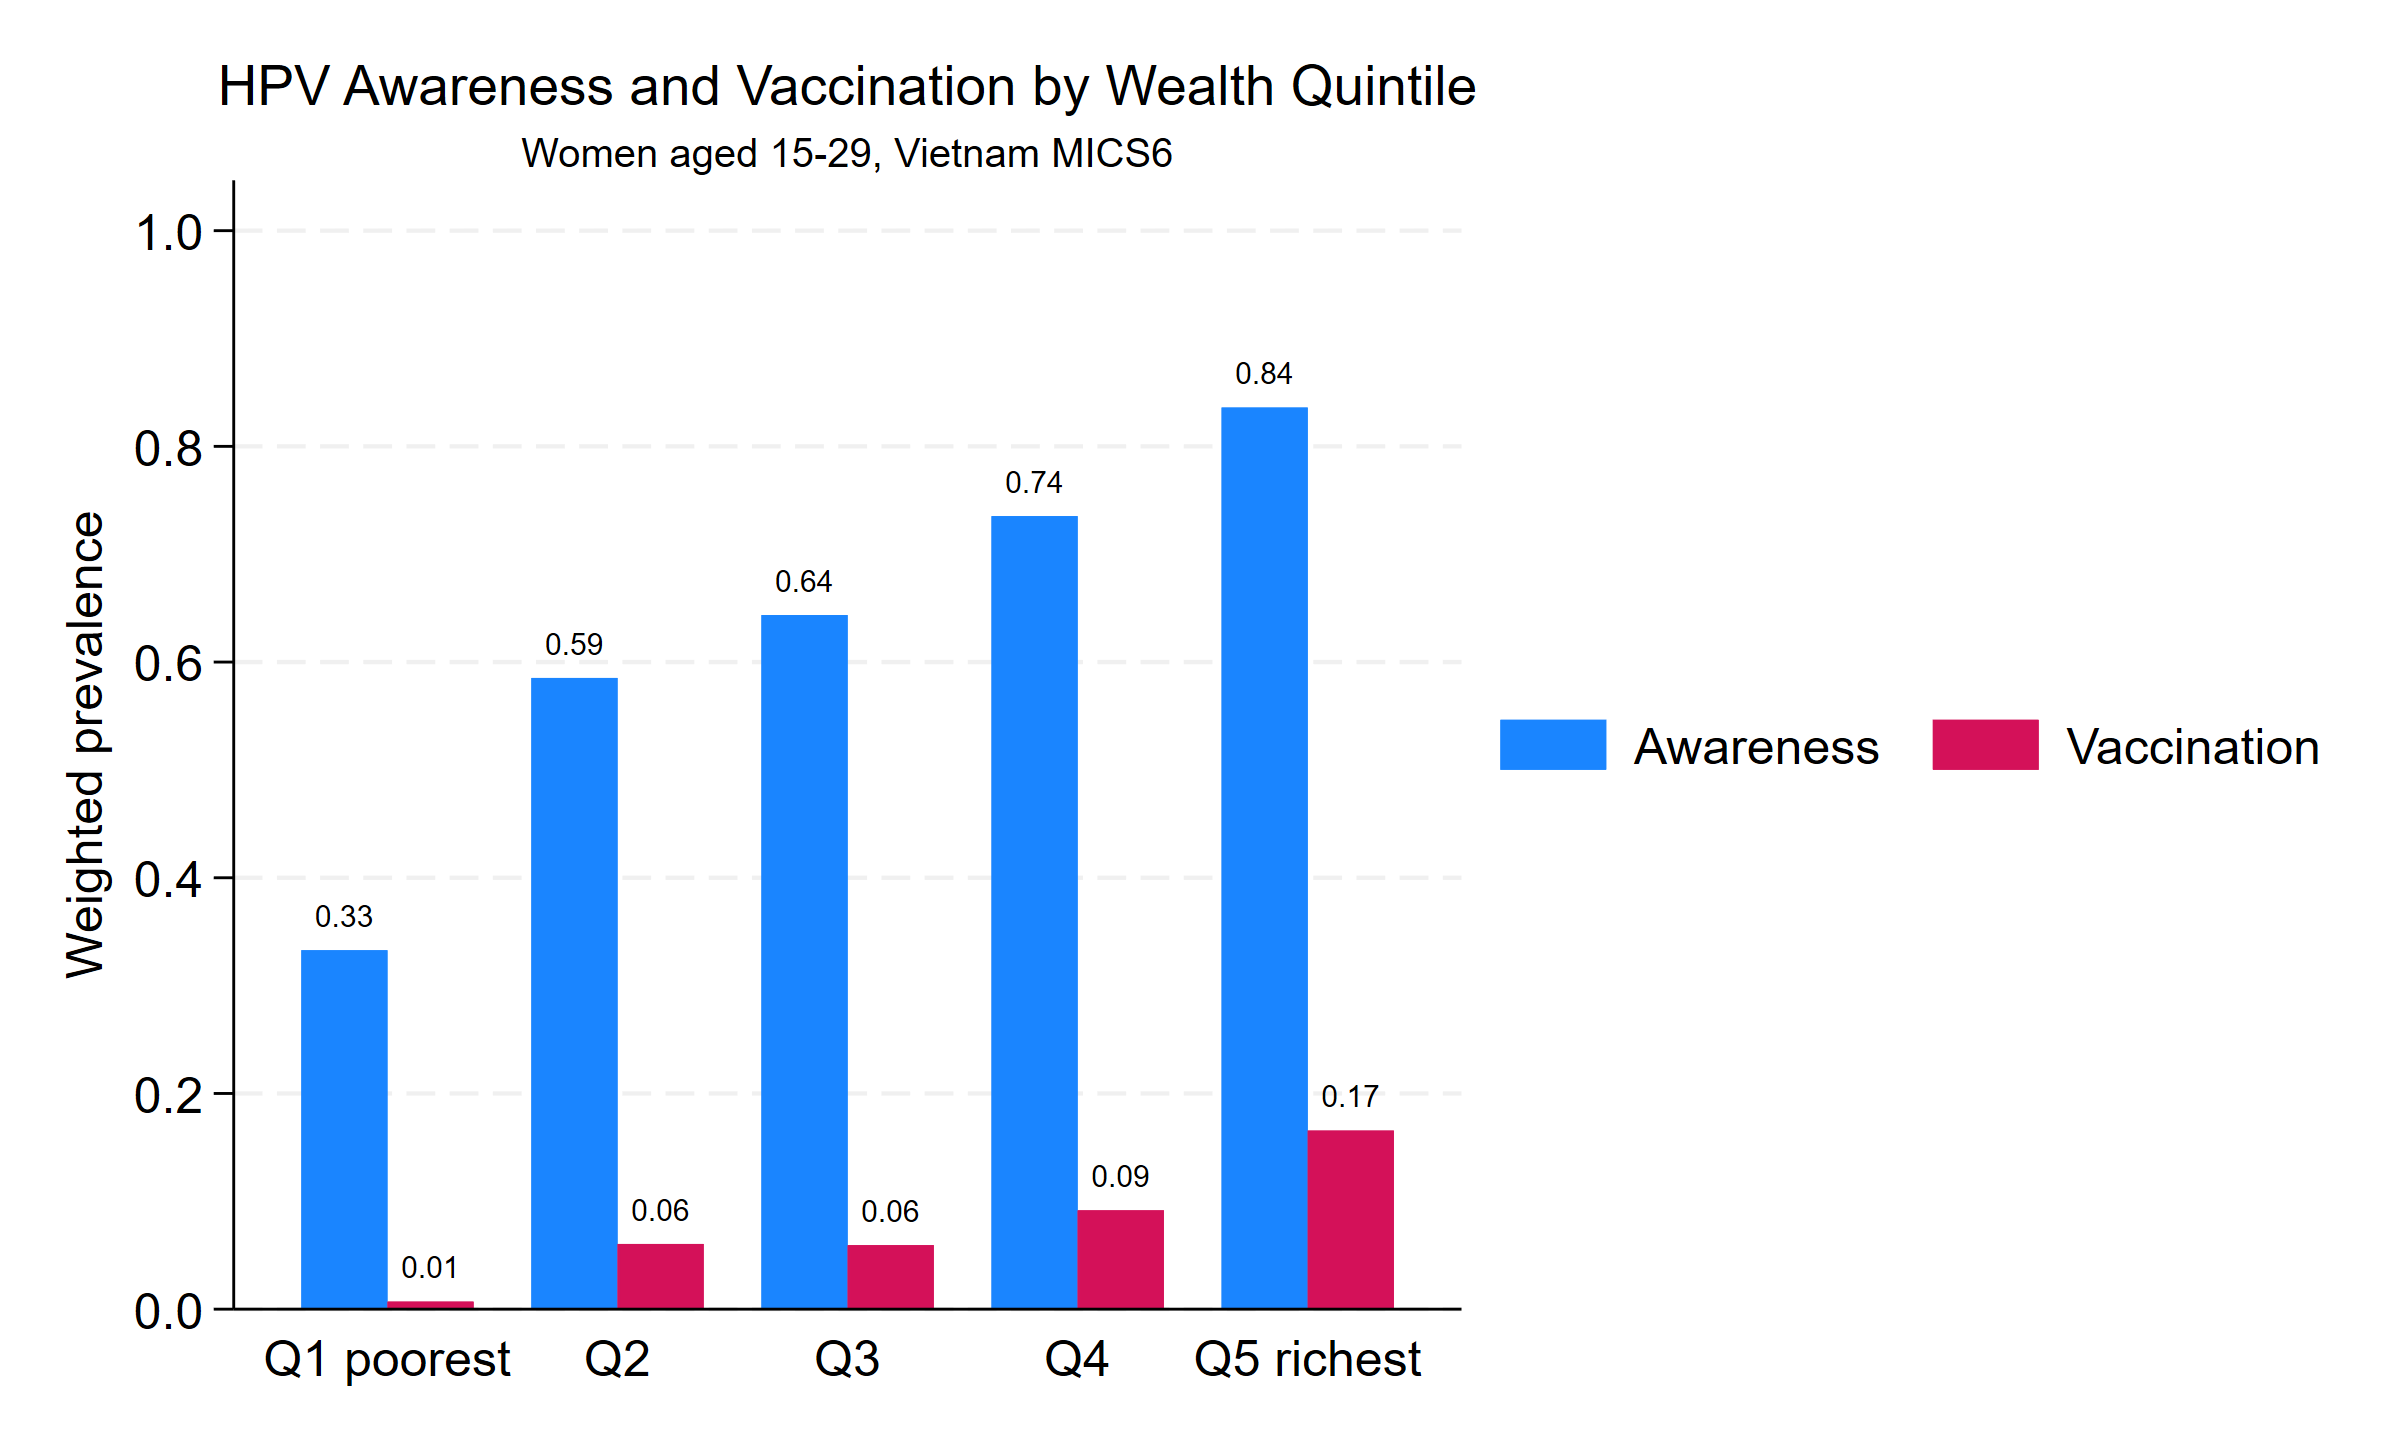
\includegraphics[width=0.90\textwidth]{Figures/fig1_awareness_vaccination_by_ses.png}
\caption{HPV vaccine awareness and vaccination prevalence by wealth quintile.}
\label{fig:awareness_vacc_ses}
\end{figure}

\begin{figure}[htbp]
\centering
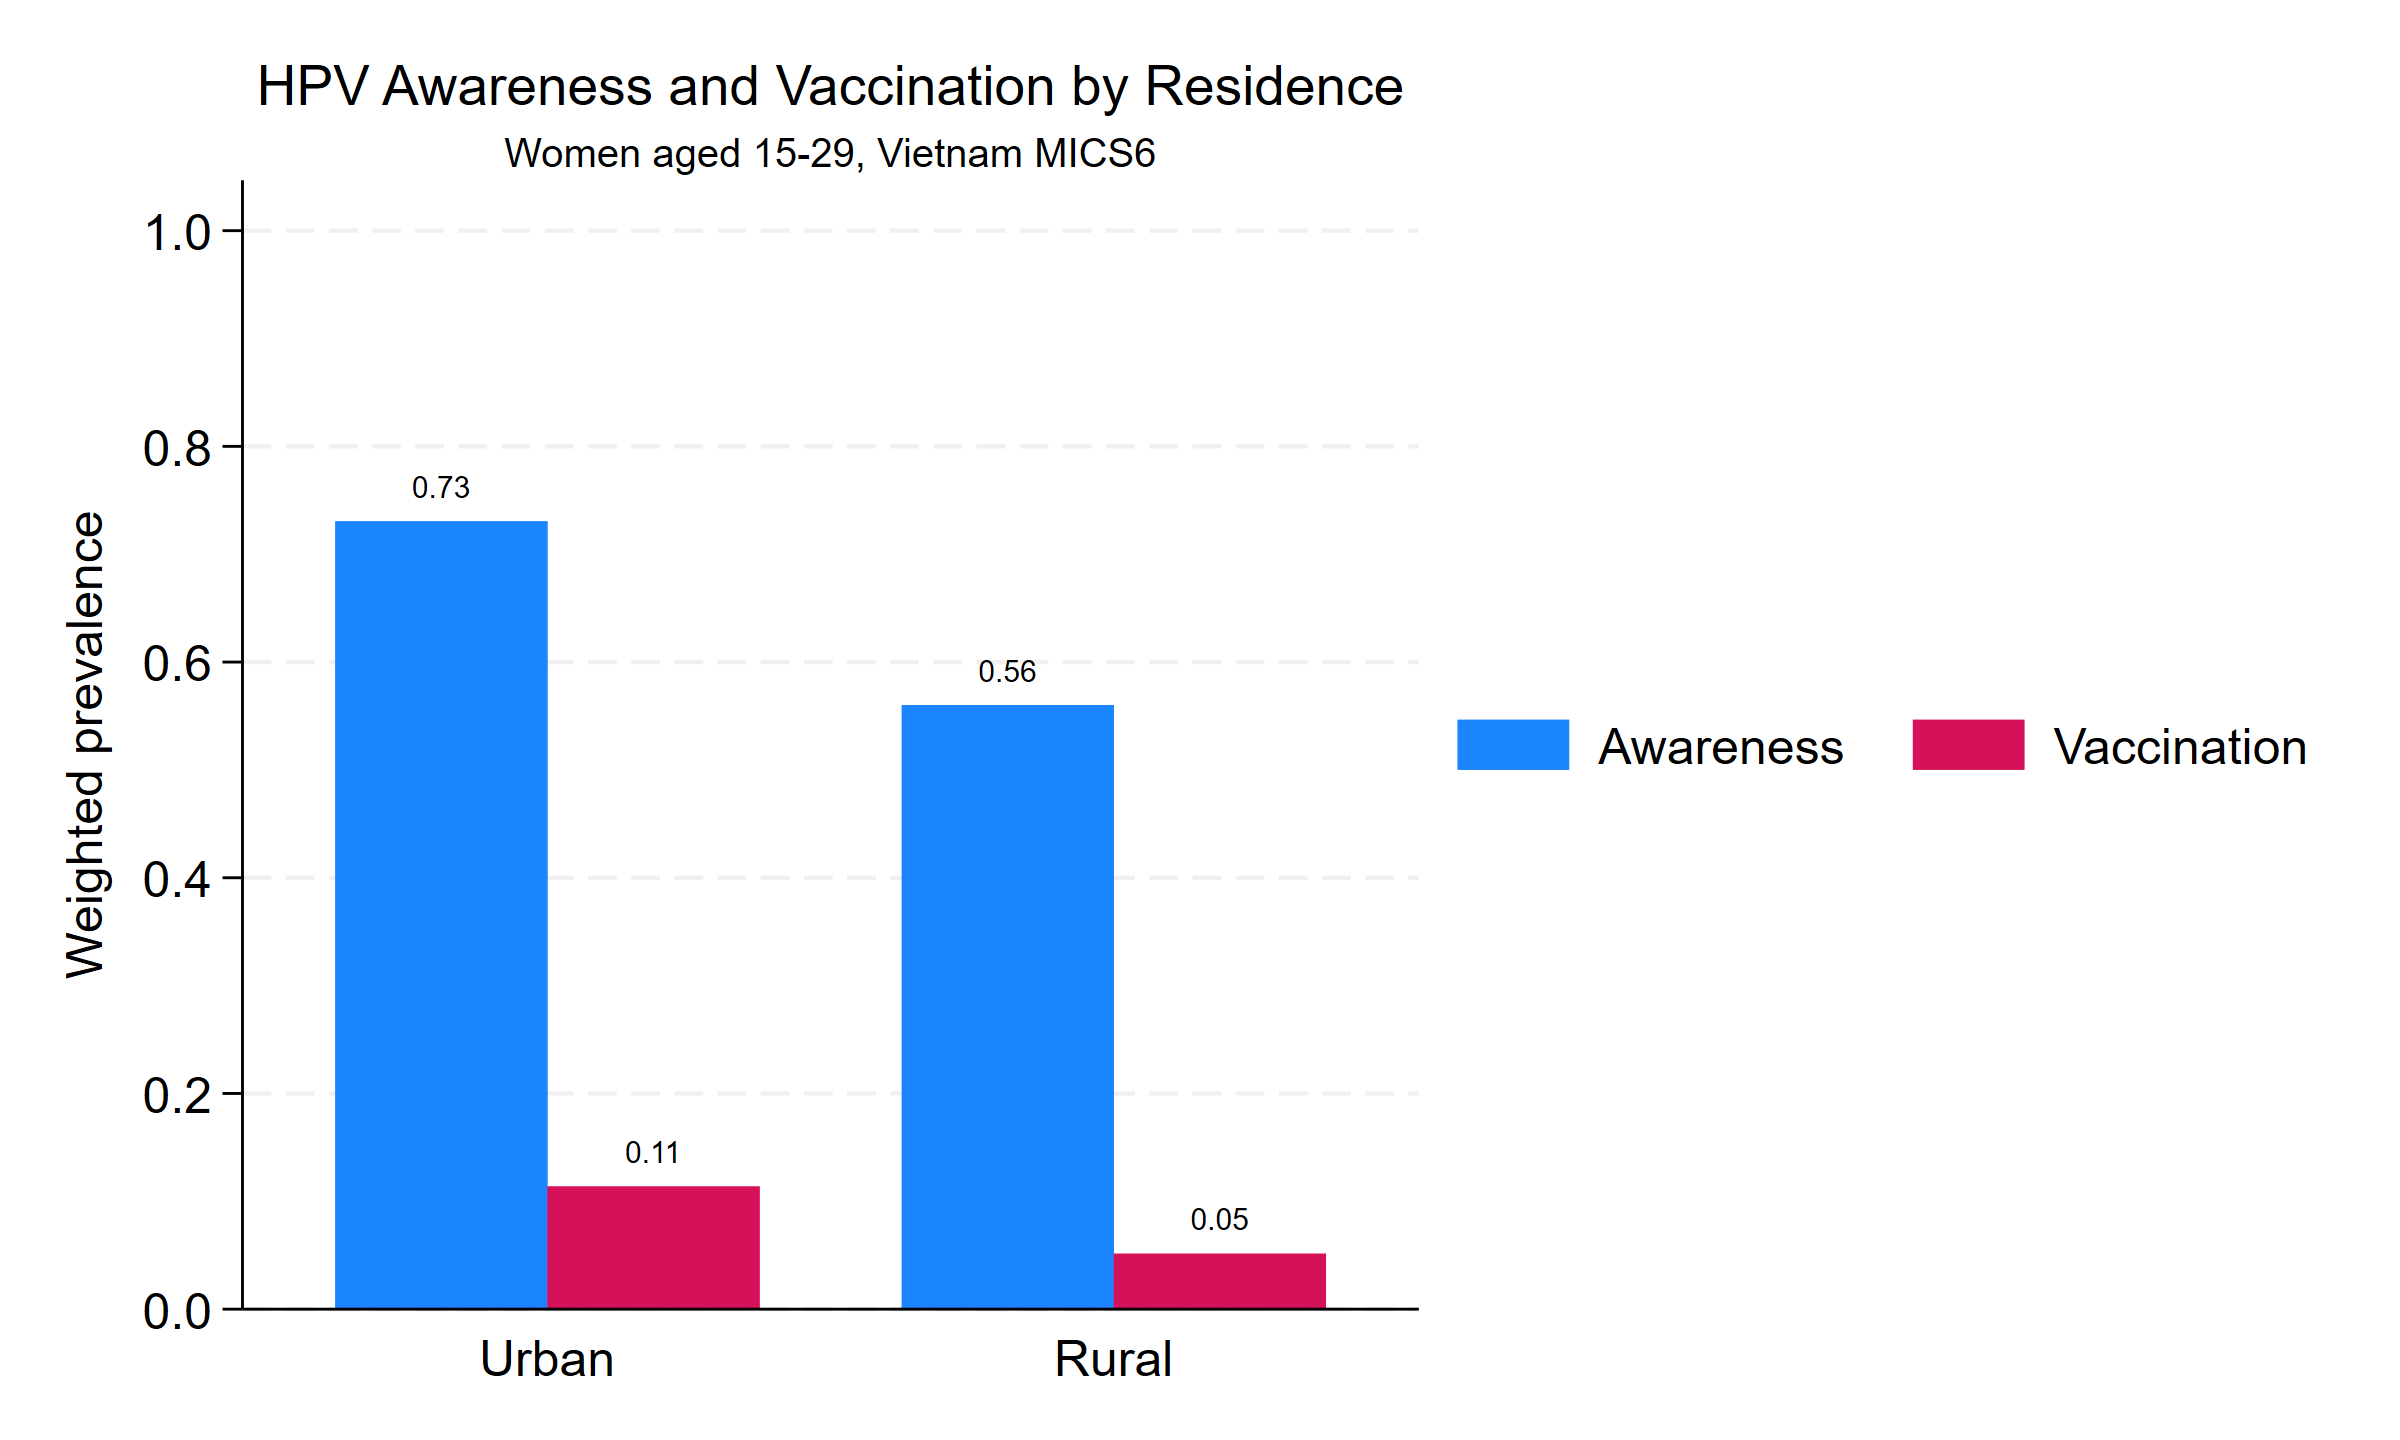
\includegraphics[width=0.88\textwidth]{Figures/fig4_awareness_vaccination_by_area.png}
\caption{HPV vaccine awareness and vaccination prevalence by urban/rural residence.}
\label{fig:awareness_vacc_area}
\end{figure}

\section{Awareness--vaccination gap}

Among women who had heard of HPV vaccination, the gap was highest among poorer and more disadvantaged groups. Table~\ref{tab:bivar_gap} presents survey-weighted gap prevalence. P-values are design-based Pearson tests using the aware subpopulation.

\begin{longtable}{|p{2.5cm}|p{2.8cm}|p{2.2cm}|p{3.2cm}|p{1.0cm}|}
\caption{Awareness--vaccination gap among women aware of HPV vaccination}
\label{tab:bivar_gap}\\
\hline
\textbf{Variable} & \textbf{Category} & \textbf{Unweighted aware n (gap n)} & \textbf{Aware but unvaccinated \% (95\% CI)} & \textbf{p} \\
\hline
\endfirsthead
\hline
\textbf{Variable} & \textbf{Category} & \textbf{Unweighted aware n (gap n)} & \textbf{Aware but unvaccinated \% (95\% CI)} & \textbf{p} \\
\hline
\endhead
Age & 15--19 & 554 (497) & 88.3 (83.9--91.7) & 0.052 \\
 & 20--24 & 623 (547) & 84.9 (80.9--88.2) &  \\
 & 25--29 & 956 (869) & 90.0 (87.4--92.1) &  \\
\hline
Residence & Urban & 855 (730) & 84.4 (80.9--87.4) & 0.002 \\
 & Rural & 1,278 (1,183) & 90.8 (88.2--92.9) &  \\
\hline
Ethnicity & Kinh/Hoa & 1,631 (1,428) & 87.3 (85.0--89.3) & 0.003 \\
 & Ethnic minority & 502 (485) & 95.5 (90.9--97.9) &  \\
\hline
Health insurance & Insured & 1,889 (1,685) & 87.3 (85.0--89.2) & 0.028 \\
 & Uninsured & 244 (228) & 93.1 (88.2--96.1) &  \\
\hline
Marital status & Currently married/union & 1,118 (1,033) & 92.0 (89.9--93.8) & $<0.001$ \\
 & Formerly married/union & 52 (44) & 86.6 (73.7--93.7) &  \\
 & Never married/union & 963 (836) & 84.3 (80.7--87.3) &  \\
\hline
Education & Primary or less & 89 (86) & 96.6 (83.7--99.4) & $<0.001$ \\
 & Lower secondary & 431 (414) & 95.1 (91.3--97.3) &  \\
 & Upper secondary+ & 1,613 (1,413) & 86.3 (83.9--88.4) &  \\
\hline
Wealth & Q1 poorest & 414 (403) & 97.9 (95.0--99.1) & $<0.001$ \\
 & Q2 & 407 (376) & 89.7 (85.0--93.0) &  \\
 & Q3 & 409 (375) & 90.8 (86.8--93.6) &  \\
 & Q4 & 446 (390) & 87.5 (83.3--90.8) &  \\
 & Q5 richest & 457 (369) & 80.2 (74.8--84.7) &  \\
\hline
Mass media & No & 149 (142) & 93.3 (83.3--97.5) & 0.195 \\
 & Yes & 1,984 (1,771) & 87.7 (85.6--89.6) &  \\
\hline
Gender-equitable attitude & No & 177 (163) & 92.8 (87.2--96.1) & 0.081 \\
 & Yes & 1,887 (1,689) & 87.9 (85.7--89.7) &  \\
\hline
Ever had sex & No & 896 (777) & 84.0 (80.3--87.1) & $<0.001$ \\
 & Yes & 1,237 (1,136) & 91.5 (89.4--93.1) &  \\
\hline
\multicolumn{5}{|p{13.0cm}|}{\footnotesize Note: Estimates use \texttt{svy, subpop(ccp5\_bin)}. P-values are descriptive design-based Pearson chi-squared tests among women who had heard of HPV vaccination and were not adjusted for multiple comparisons.} \\
\hline
\end{longtable}

\begin{figure}[htbp]
\centering
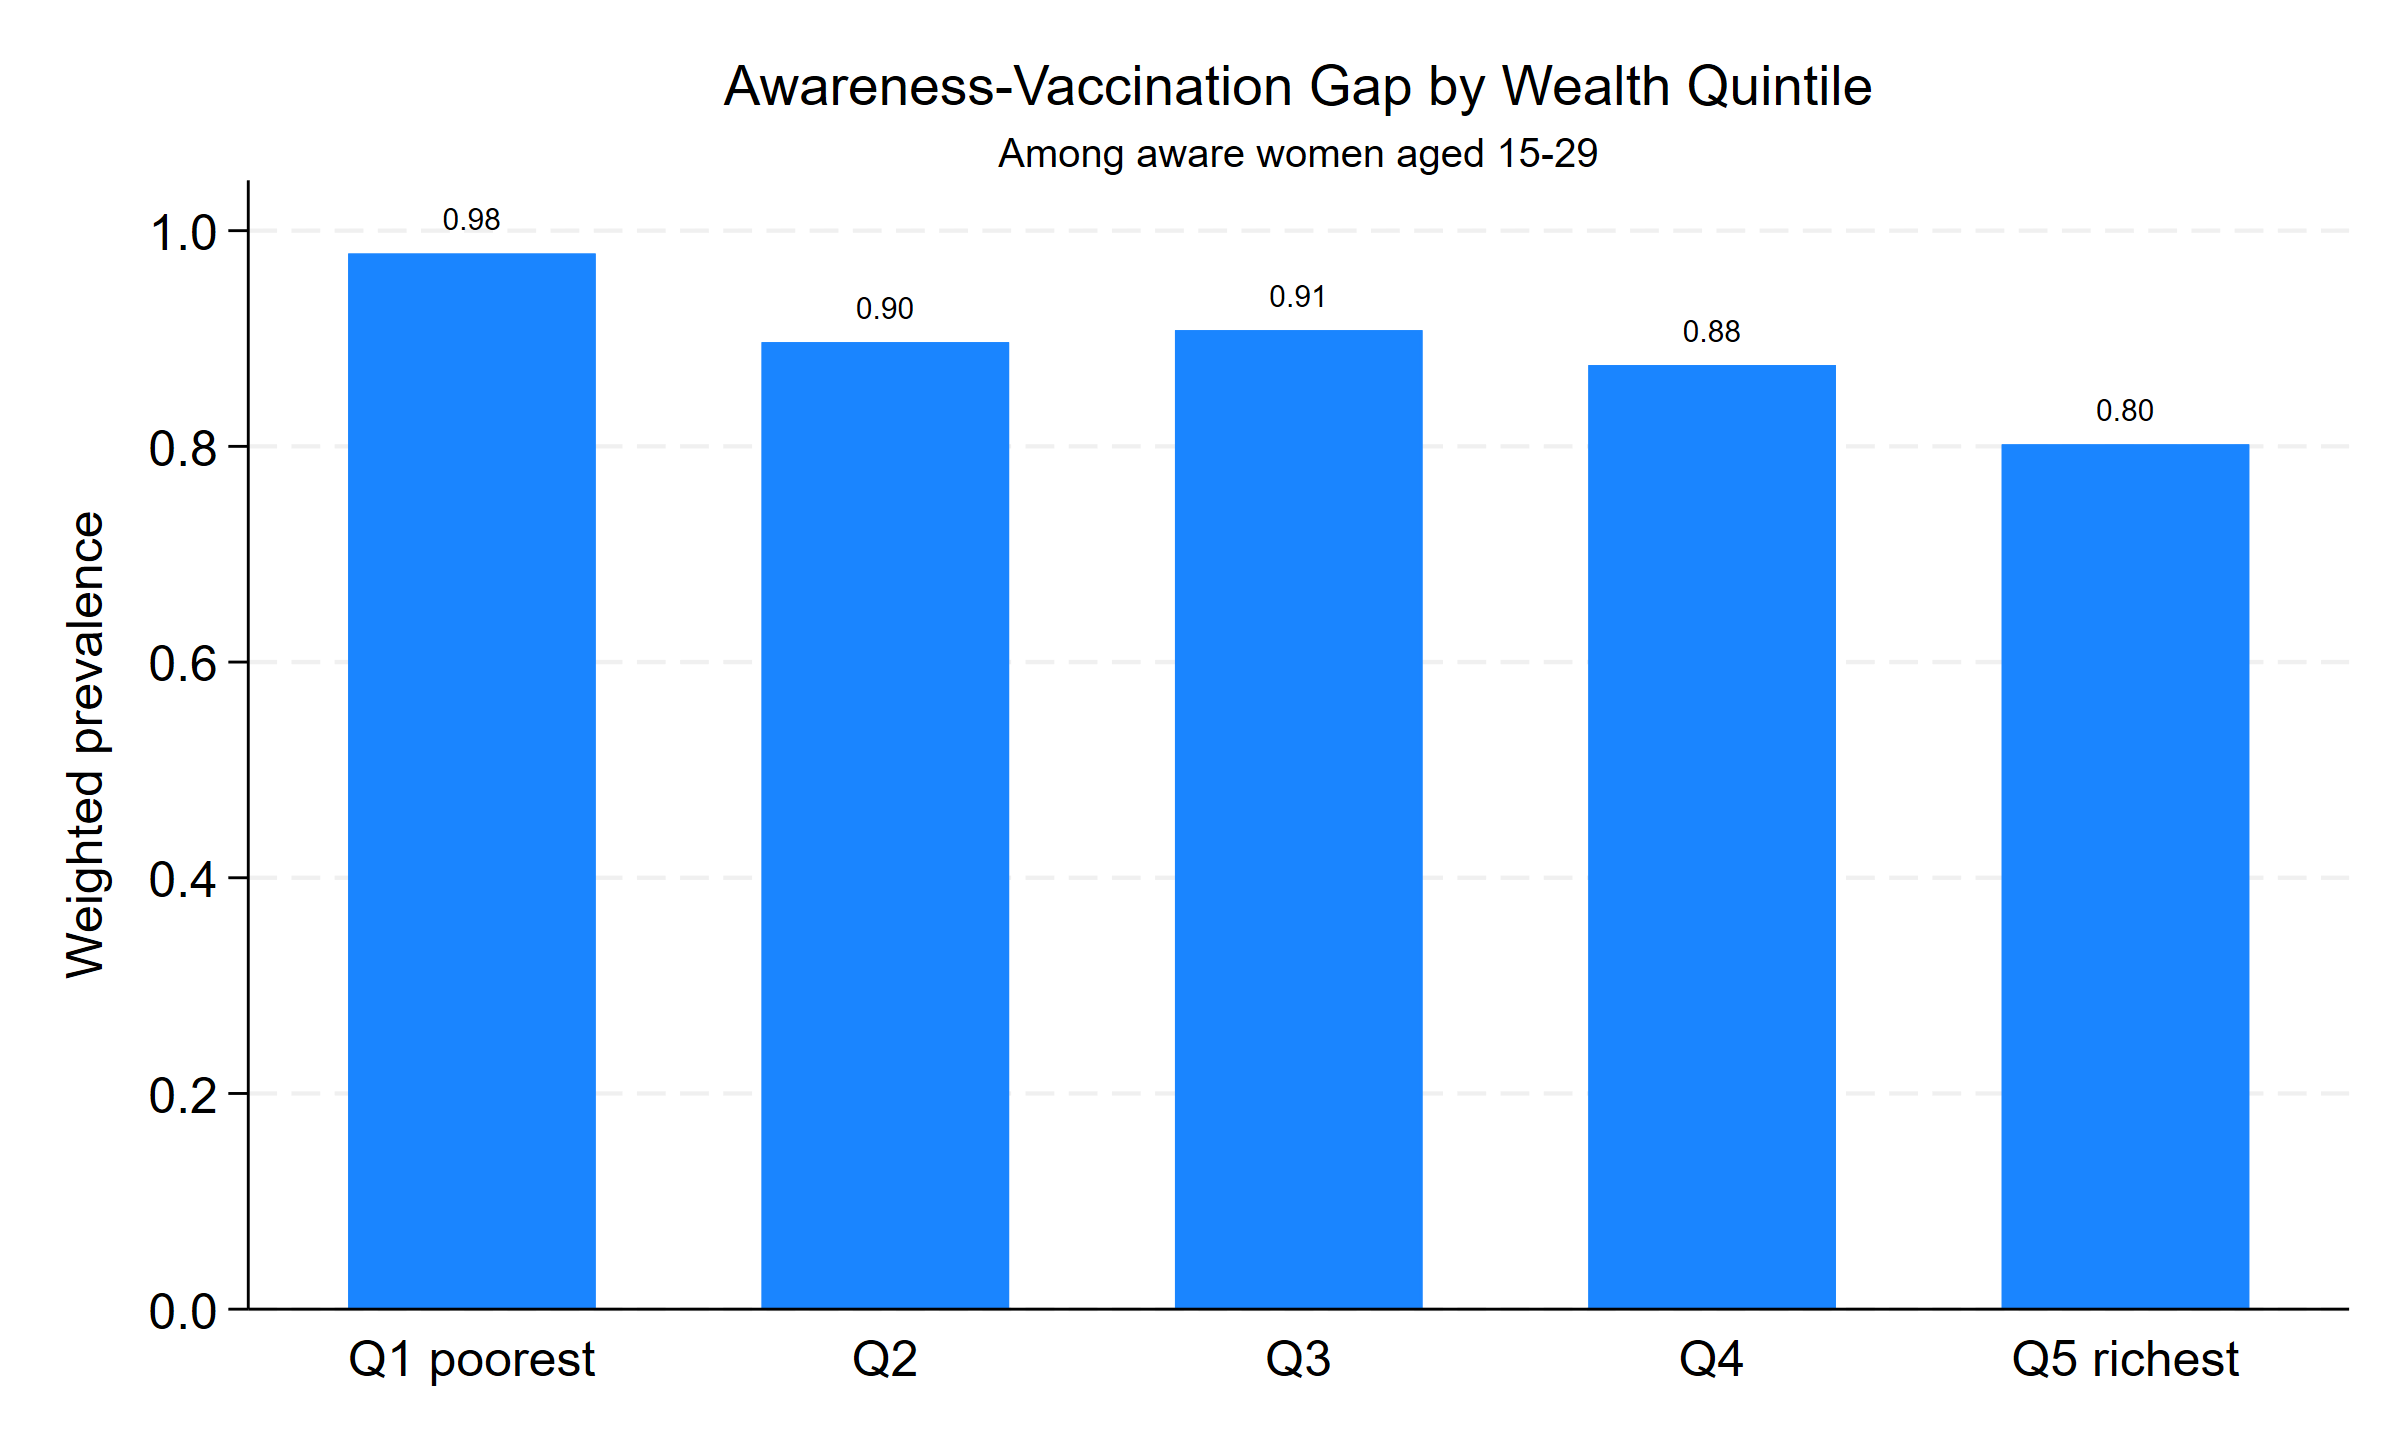
\includegraphics[width=0.88\textwidth]{Figures/fig2_gap_by_ses.png}
\caption{Awareness--vaccination gap by wealth quintile among women who had heard of HPV vaccination.}
\label{fig:gap_ses}
\end{figure}

\section{Socioeconomic inequality}

Both awareness and vaccination were pro-rich. Vaccination showed stronger relative socioeconomic concentration than awareness based on the standard concentration index: 0.389 (95\% CI: 0.296--0.482) for vaccination compared with 0.149 (95\% CI: 0.131--0.166) for awareness. Erreygers-corrected indices should be interpreted as absolute inequality measures for bounded outcomes and are influenced by outcome prevalence; these were 0.371 (95\% CI: 0.328--0.415) for awareness and 0.116 (95\% CI: 0.089--0.144) for vaccination. The gap had a negative concentration index, showing that, among aware women, being unvaccinated was concentrated among poorer women.

\begin{table}[htbp]
\caption[Concentration indices]{Concentration indices for HPV vaccine awareness, vaccination, and awareness--vaccination gap}
\centering
\small
\begin{tabular}{|p{4.2cm}|c|c|c|c|}
\hline
\textbf{Outcome} & \textbf{Index} & \textbf{N} & \textbf{Estimate (95\% CI)} & \textbf{p} \\
\hline
Awareness & Standard CI & 4,102 & 0.149 (0.131--0.166) & $<0.001$ \\
Awareness & Erreygers CI & 4,102 & 0.371 (0.328--0.415) & $<0.001$ \\
\hline
Vaccination & Standard CI & 4,102 & 0.389 (0.296--0.482) & $<0.001$ \\
Vaccination & Erreygers CI & 4,102 & 0.116 (0.089--0.144) & $<0.001$ \\
\hline
Gap & Standard CI & 2,133 & -0.035 (-0.047 to -0.023) & $<0.001$ \\
Gap & Erreygers CI & 2,133 & -0.123 (-0.164 to -0.082) & $<0.001$ \\
\hline
\multicolumn{5}{|p{13.0cm}|}{\footnotesize Note: Ranking variable was the continuous household wealth score. Estimates used the survey design. Positive values indicate pro-rich concentration; negative values indicate pro-poor concentration.} \\
\hline
\end{tabular}
\label{tab:concentration}
\end{table}

\begin{figure}[htbp]
\centering
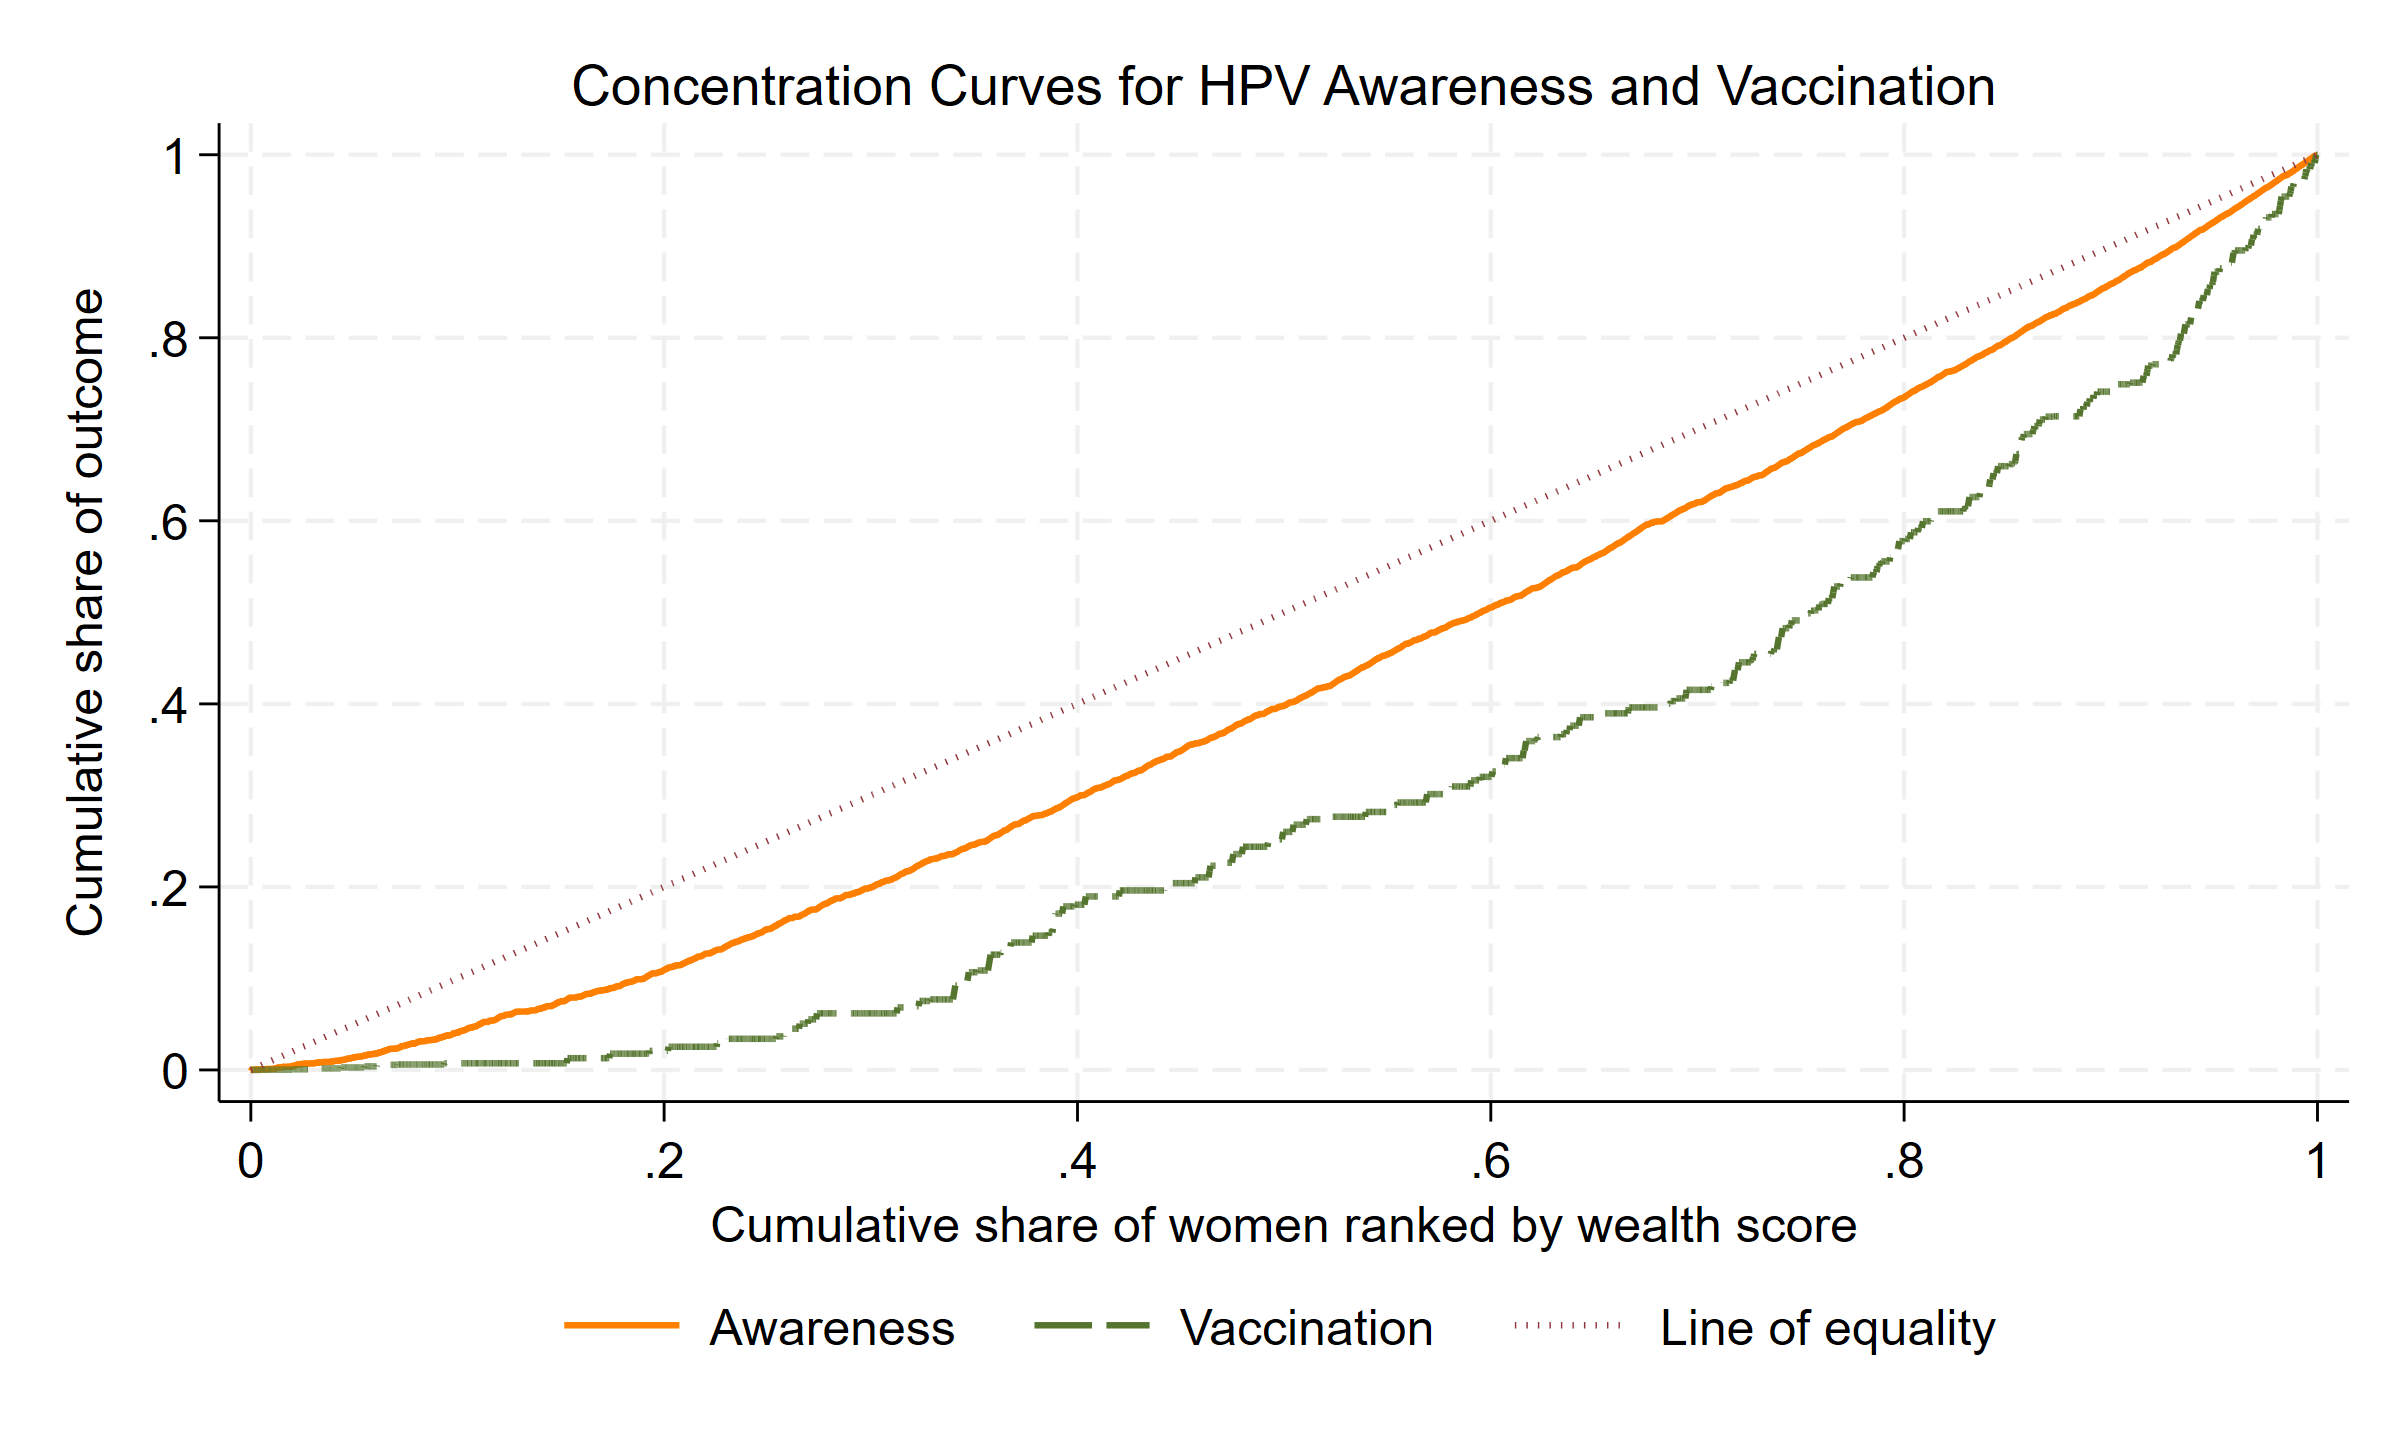
\includegraphics[width=0.88\textwidth]{Figures/fig7_concentration_curve.png}
\caption{Concentration curves for HPV vaccine awareness and vaccination ranked by household wealth score.}
\label{fig:concentration_curves}
\end{figure}

\section{Adjusted regression models}

Tables~\ref{tab:adjusted_awareness}--\ref{tab:adjusted_gap} present survey-weighted Poisson regression models. All estimates are adjusted prevalence ratios. The awareness and vaccination models used the full analytic sample with complete model covariates (N~=~3,899). The gap model used the aware subpopulation while preserving the survey design (N~=~4,033 in the design sample; subpopulation observations were aware women with complete model covariates). P-values are model-based t-tests from survey-weighted Poisson regression with Taylor linearized survey variance.

\begin{longtable}{|p{6.2cm}|p{3.6cm}|p{1.3cm}|}
\caption{Adjusted prevalence ratios for HPV vaccine awareness}
\label{tab:adjusted_awareness}\\
\hline
\textbf{Variable} & \textbf{Awareness aPR (95\% CI)} & \textbf{p} \\
\hline
\endfirsthead
\hline
\textbf{Variable} & \textbf{Awareness aPR (95\% CI)} & \textbf{p} \\
\hline
\endhead
Rural (ref: urban) & 0.933 (0.867--1.005) & 0.068 \\
Age 15--19 (ref: 25--29) & \textbf{0.626 (0.561--0.699)} & $<0.001$ \\
Age 20--24 (ref: 25--29) & \textbf{0.918 (0.855--0.986)} & 0.019 \\
Formerly married/union (ref: current) & 0.882 (0.730--1.065) & 0.192 \\
Never married/union (ref: current) & 1.050 (0.868--1.270) & 0.615 \\
Primary or less (ref: upper secondary+) & \textbf{0.475 (0.330--0.683)} & $<0.001$ \\
Lower secondary (ref: upper secondary+) & \textbf{0.836 (0.754--0.927)} & $<0.001$ \\
Uninsured (ref: insured) & 0.997 (0.898--1.108) & 0.962 \\
Ethnic minority (ref: Kinh/Hoa) & \textbf{0.860 (0.745--0.992)} & 0.038 \\
Q1 poorest (ref: Q5 richest) & \textbf{0.576 (0.480--0.691)} & $<0.001$ \\
Q2 (ref: Q5 richest) & \textbf{0.802 (0.726--0.885)} & $<0.001$ \\
Q3 (ref: Q5 richest) & \textbf{0.812 (0.743--0.888)} & $<0.001$ \\
Q4 (ref: Q5 richest) & \textbf{0.890 (0.829--0.956)} & 0.001 \\
Mass media exposure (ref: no) & 1.147 (0.981--1.340) & 0.084 \\
Rejects all wife-beating justifications (ref: no) & \textbf{1.234 (1.066--1.429)} & 0.005 \\
Ever had sexual intercourse (ref: no) & 1.024 (0.857--1.224) & 0.793 \\
\hline
\multicolumn{3}{|p{11.6cm}|}{\footnotesize Model N = 3,899. Reference categories: urban, age 25--29, currently married/in union, upper secondary or higher, insured, Kinh/Hoa, Q5 richest, no mass media exposure, no gender-equitable attitude proxy, and never had sexual intercourse. Bold estimates have p < 0.05. ICT was excluded because weighted prevalence was 97.9\%.} \\
\hline
\end{longtable}

\begin{longtable}{|p{6.2cm}|p{3.6cm}|p{1.3cm}|}
\caption{Adjusted prevalence ratios for self-reported any-dose HPV vaccine uptake}
\label{tab:adjusted_vaccination}\\
\hline
\textbf{Variable} & \textbf{Any-dose uptake aPR (95\% CI)} & \textbf{p} \\
\hline
\endfirsthead
\hline
\textbf{Variable} & \textbf{Any-dose uptake aPR (95\% CI)} & \textbf{p} \\
\hline
\endhead
Rural (ref: urban) & 0.780 (0.547--1.112) & 0.169 \\
Age 15--19 (ref: 25--29) & \textbf{0.514 (0.305--0.865)} & 0.012 \\
Age 20--24 (ref: 25--29) & 1.150 (0.796--1.660) & 0.456 \\
Formerly married/union (ref: current) & 1.482 (0.697--3.150) & 0.306 \\
Never married/union (ref: current) & 1.195 (0.578--2.470) & 0.631 \\
Primary or less (ref: upper secondary+) & 0.327 (0.060--1.770) & 0.194 \\
Lower secondary (ref: upper secondary+) & \textbf{0.422 (0.227--0.785)} & 0.007 \\
Uninsured (ref: insured) & 0.676 (0.381--1.197) & 0.179 \\
Ethnic minority (ref: Kinh/Hoa) & 0.743 (0.307--1.801) & 0.510 \\
Q1 poorest (ref: Q5 richest) & \textbf{0.118 (0.039--0.358)} & $<0.001$ \\
Q2 (ref: Q5 richest) & \textbf{0.585 (0.365--0.936)} & 0.026 \\
Q3 (ref: Q5 richest) & \textbf{0.437 (0.278--0.688)} & $<0.001$ \\
Q4 (ref: Q5 richest) & \textbf{0.631 (0.421--0.945)} & 0.026 \\
Mass media exposure (ref: no) & 1.960 (0.763--5.034) & 0.162 \\
Rejects all wife-beating justifications (ref: no) & 1.614 (0.861--3.025) & 0.135 \\
Ever had sexual intercourse (ref: no) & 0.739 (0.352--1.550) & 0.423 \\
\hline
\multicolumn{3}{|p{11.6cm}|}{\footnotesize Model N = 3,899. Reference categories: urban, age 25--29, currently married/in union, upper secondary or higher, insured, Kinh/Hoa, Q5 richest, no mass media exposure, no gender-equitable attitude proxy, and never had sexual intercourse. Bold estimates have p < 0.05. ICT was excluded because weighted prevalence was 97.9\%.} \\
\hline
\end{longtable}

\begin{longtable}{|p{6.2cm}|p{3.6cm}|p{1.3cm}|}
\caption{Adjusted prevalence ratios for awareness--vaccination gap among aware women}
\label{tab:adjusted_gap}\\
\hline
\textbf{Variable} & \textbf{Gap PR (95\% CI)} & \textbf{p} \\
\hline
\endfirsthead
\hline
\textbf{Variable} & \textbf{Gap PR (95\% CI)} & \textbf{p} \\
\hline
\endhead
Rural (ref: urban) & 1.024 (0.976--1.075) & 0.331 \\
Age 15--19 (ref: 25--29) & 1.053 (0.979--1.134) & 0.166 \\
Age 20--24 (ref: 25--29) & 0.975 (0.929--1.023) & 0.299 \\
Formerly married/union (ref: current) & 0.955 (0.856--1.066) & 0.412 \\
Never married/union (ref: current) & 0.973 (0.886--1.069) & 0.568 \\
Primary or less (ref: upper secondary+) & 1.008 (0.940--1.081) & 0.816 \\
Lower secondary (ref: upper secondary+) & \textbf{1.041 (1.003--1.081)} & 0.036 \\
Uninsured (ref: insured) & 1.039 (0.991--1.090) & 0.112 \\
Ethnic minority (ref: Kinh/Hoa) & 1.010 (0.957--1.066) & 0.716 \\
Q1 poorest (ref: Q5 richest) & \textbf{1.137 (1.055--1.225)} & $<0.001$ \\
Q2 (ref: Q5 richest) & 1.070 (0.992--1.154) & 0.079 \\
Q3 (ref: Q5 richest) & \textbf{1.104 (1.028--1.185)} & 0.007 \\
Q4 (ref: Q5 richest) & 1.073 (0.994--1.158) & 0.069 \\
Mass media exposure (ref: no) & 0.962 (0.919--1.007) & 0.097 \\
Rejects all wife-beating justifications (ref: no) & 0.978 (0.929--1.029) & 0.391 \\
Ever had sexual intercourse (ref: no) & 1.050 (0.945--1.166) & 0.361 \\
\hline
\multicolumn{3}{|p{11.6cm}|}{\footnotesize Model N = 4,033. Reference categories: urban, age 25--29, currently married/in union, upper secondary or higher, insured, Kinh/Hoa, Q5 richest, no mass media exposure, no gender-equitable attitude proxy, and never had sexual intercourse. Bold estimates have p < 0.05. ICT was excluded because weighted prevalence was 97.9\%.} \\
\hline
\end{longtable}

After adjustment, wealth remained a consistent marker of the awareness-to-uptake pathway. Compared with the richest quintile, the poorest quintile had 42\% lower awareness and 88\% lower vaccination prevalence. Among aware women, the poorest quintile had a higher prevalence of remaining unvaccinated. Lower secondary education was associated with lower vaccination and a higher gap. The gender-equitable attitude proxy was independently associated with higher awareness but not with vaccination after adjustment.

\section{Absolute differences and vaccination among aware women}

Because vaccination was rare in the poorest quintile and the gap outcome was very common, absolute differences help interpret the relative models. In bivariate survey-weighted estimates among women who had heard of HPV vaccination, vaccination increased from 2.1\% in the poorest quintile (95\% CI: 0.9--5.0) to 19.8\% in the richest quintile (95\% CI: 15.3--25.2), with a design-based Pearson p-value $<0.001$. This sensitivity analysis shows that wealth differences persist even after conditioning on awareness.

Table~\ref{tab:predicted_wealth} reports adjusted predicted probabilities from survey-weighted logistic models. Compared with the richest quintile, the poorest quintile had a 31.5 percentage-point lower adjusted probability of awareness, a 10.8 percentage-point lower adjusted probability of vaccination in the full analytic sample, and an 11.8 percentage-point lower adjusted probability of vaccination among aware women. The adjusted gap probability was 11.8 percentage points higher in the poorest quintile than in the richest quintile.

\begin{table}[H]
\caption{Adjusted predicted probabilities by wealth quintile}
\centering
\small
\setlength{\tabcolsep}{2pt}
\begin{tabular}{|p{2.1cm}|p{2.45cm}|p{2.45cm}|p{2.65cm}|p{2.45cm}|}
\hline
\textbf{Wealth} & \textbf{Aware \% (95\% CI)} & \textbf{Vaccinated \% (95\% CI)} & \textbf{Vaccinated if aware \% (95\% CI)} & \textbf{Gap \% (95\% CI)} \\
\hline
Q1 poorest & 48.0 (41.2--54.9) & 1.5 (0.0--3.1) & 3.1 (0.0--6.2) & 96.9 (93.8--100.0) \\
Q2 & 61.1 (56.6--65.7) & 7.1 (4.4--9.8) & 11.1 (7.0--15.2) & 88.9 (84.8--93.0) \\
Q3 & 61.8 (56.7--66.8) & 5.3 (3.4--7.2) & 8.3 (5.2--11.4) & 91.7 (88.6--94.8) \\
Q4 & 68.6 (63.7--73.6) & 7.7 (5.2--10.1) & 10.4 (7.0--13.8) & 89.6 (86.2--93.0) \\
Q5 richest & 79.5 (74.9--84.1) & 12.3 (8.8--15.7) & 15.0 (10.7--19.2) & 85.0 (80.8--89.3) \\
\hline
\multicolumn{5}{|p{12.1cm}|}{\footnotesize Note: Estimates are adjusted predicted probabilities from survey-weighted logistic regression models with the same covariates as the primary Poisson models. Gap and vaccination-among-aware models used the aware subpopulation while preserving the survey design. Confidence interval bounds for probabilities are shown within the 0--100\% scale.} \\
\hline
\end{tabular}
\label{tab:predicted_wealth}
\end{table}

\section{Erreygers decomposition}

Decomposition results are summarized in Table~\ref{tab:decomp}. Percentages indicate each determinant's contribution to the total Erreygers concentration index. Positive percentage values contribute in the direction of the total index; negative values offset it.

\begin{table}[htbp]
\caption{Main contributors to Erreygers inequality decomposition}
\centering
\small
\begin{tabular}{|p{3.7cm}|p{3.0cm}|c|c|}
\hline
\textbf{Outcome} & \textbf{Contributor} & \textbf{Contribution} & \textbf{\% of total} \\
\hline
\multirow{7}{*}{Awareness} & Q1 poorest & 0.1854 & 50.0 \\
 & Q2 & 0.0649 & 17.5 \\
 & Primary or less & 0.0372 & 10.0 \\
 & Lower secondary & 0.0326 & 8.8 \\
 & Ethnic minority & 0.0265 & 7.1 \\
 & Rural residence & 0.0205 & 5.5 \\
 & Residual & 0.0285 & 7.7 \\
\hline
\multirow{7}{*}{Vaccination} & Q1 poorest & 0.0770 & 66.1 \\
 & Lower secondary & 0.0164 & 14.1 \\
 & Q2 & 0.0154 & 13.2 \\
 & Q4 & -0.0132 & -11.3 \\
 & Primary or less & 0.0093 & 8.0 \\
 & Rural residence & 0.0079 & 6.8 \\
 & Residual & -0.0203 & -17.4 \\
\hline
\multirow{7}{*}{Gap} & Q1 poorest & -0.0546 & 44.4 \\
 & Lower secondary & -0.0200 & 16.2 \\
 & Q2 & -0.0188 & 15.2 \\
 & Q4 & 0.0121 & -9.9 \\
 & Q3 & -0.0109 & 8.8 \\
 & Rural residence & -0.0076 & 6.2 \\
 & Residual & 0.0007 & -0.6 \\
\hline
\multicolumn{4}{|p{13.0cm}|}{\footnotesize Note: Decomposition used dummy-coded covariates, probit average marginal effects, and survey-weighted standard concentration indices for each determinant; contributions sum to the Erreygers concentration index of each outcome plus a residual. Reference groups match the adjusted models. Bootstrap confidence intervals were not estimated; contributions should be interpreted as explanatory accounting rather than causal attribution. Full output is available in the generated Stata CSV file.} \\
\hline
\end{tabular}
\label{tab:decomp}
\end{table}

\begin{figure}[htbp]
\centering
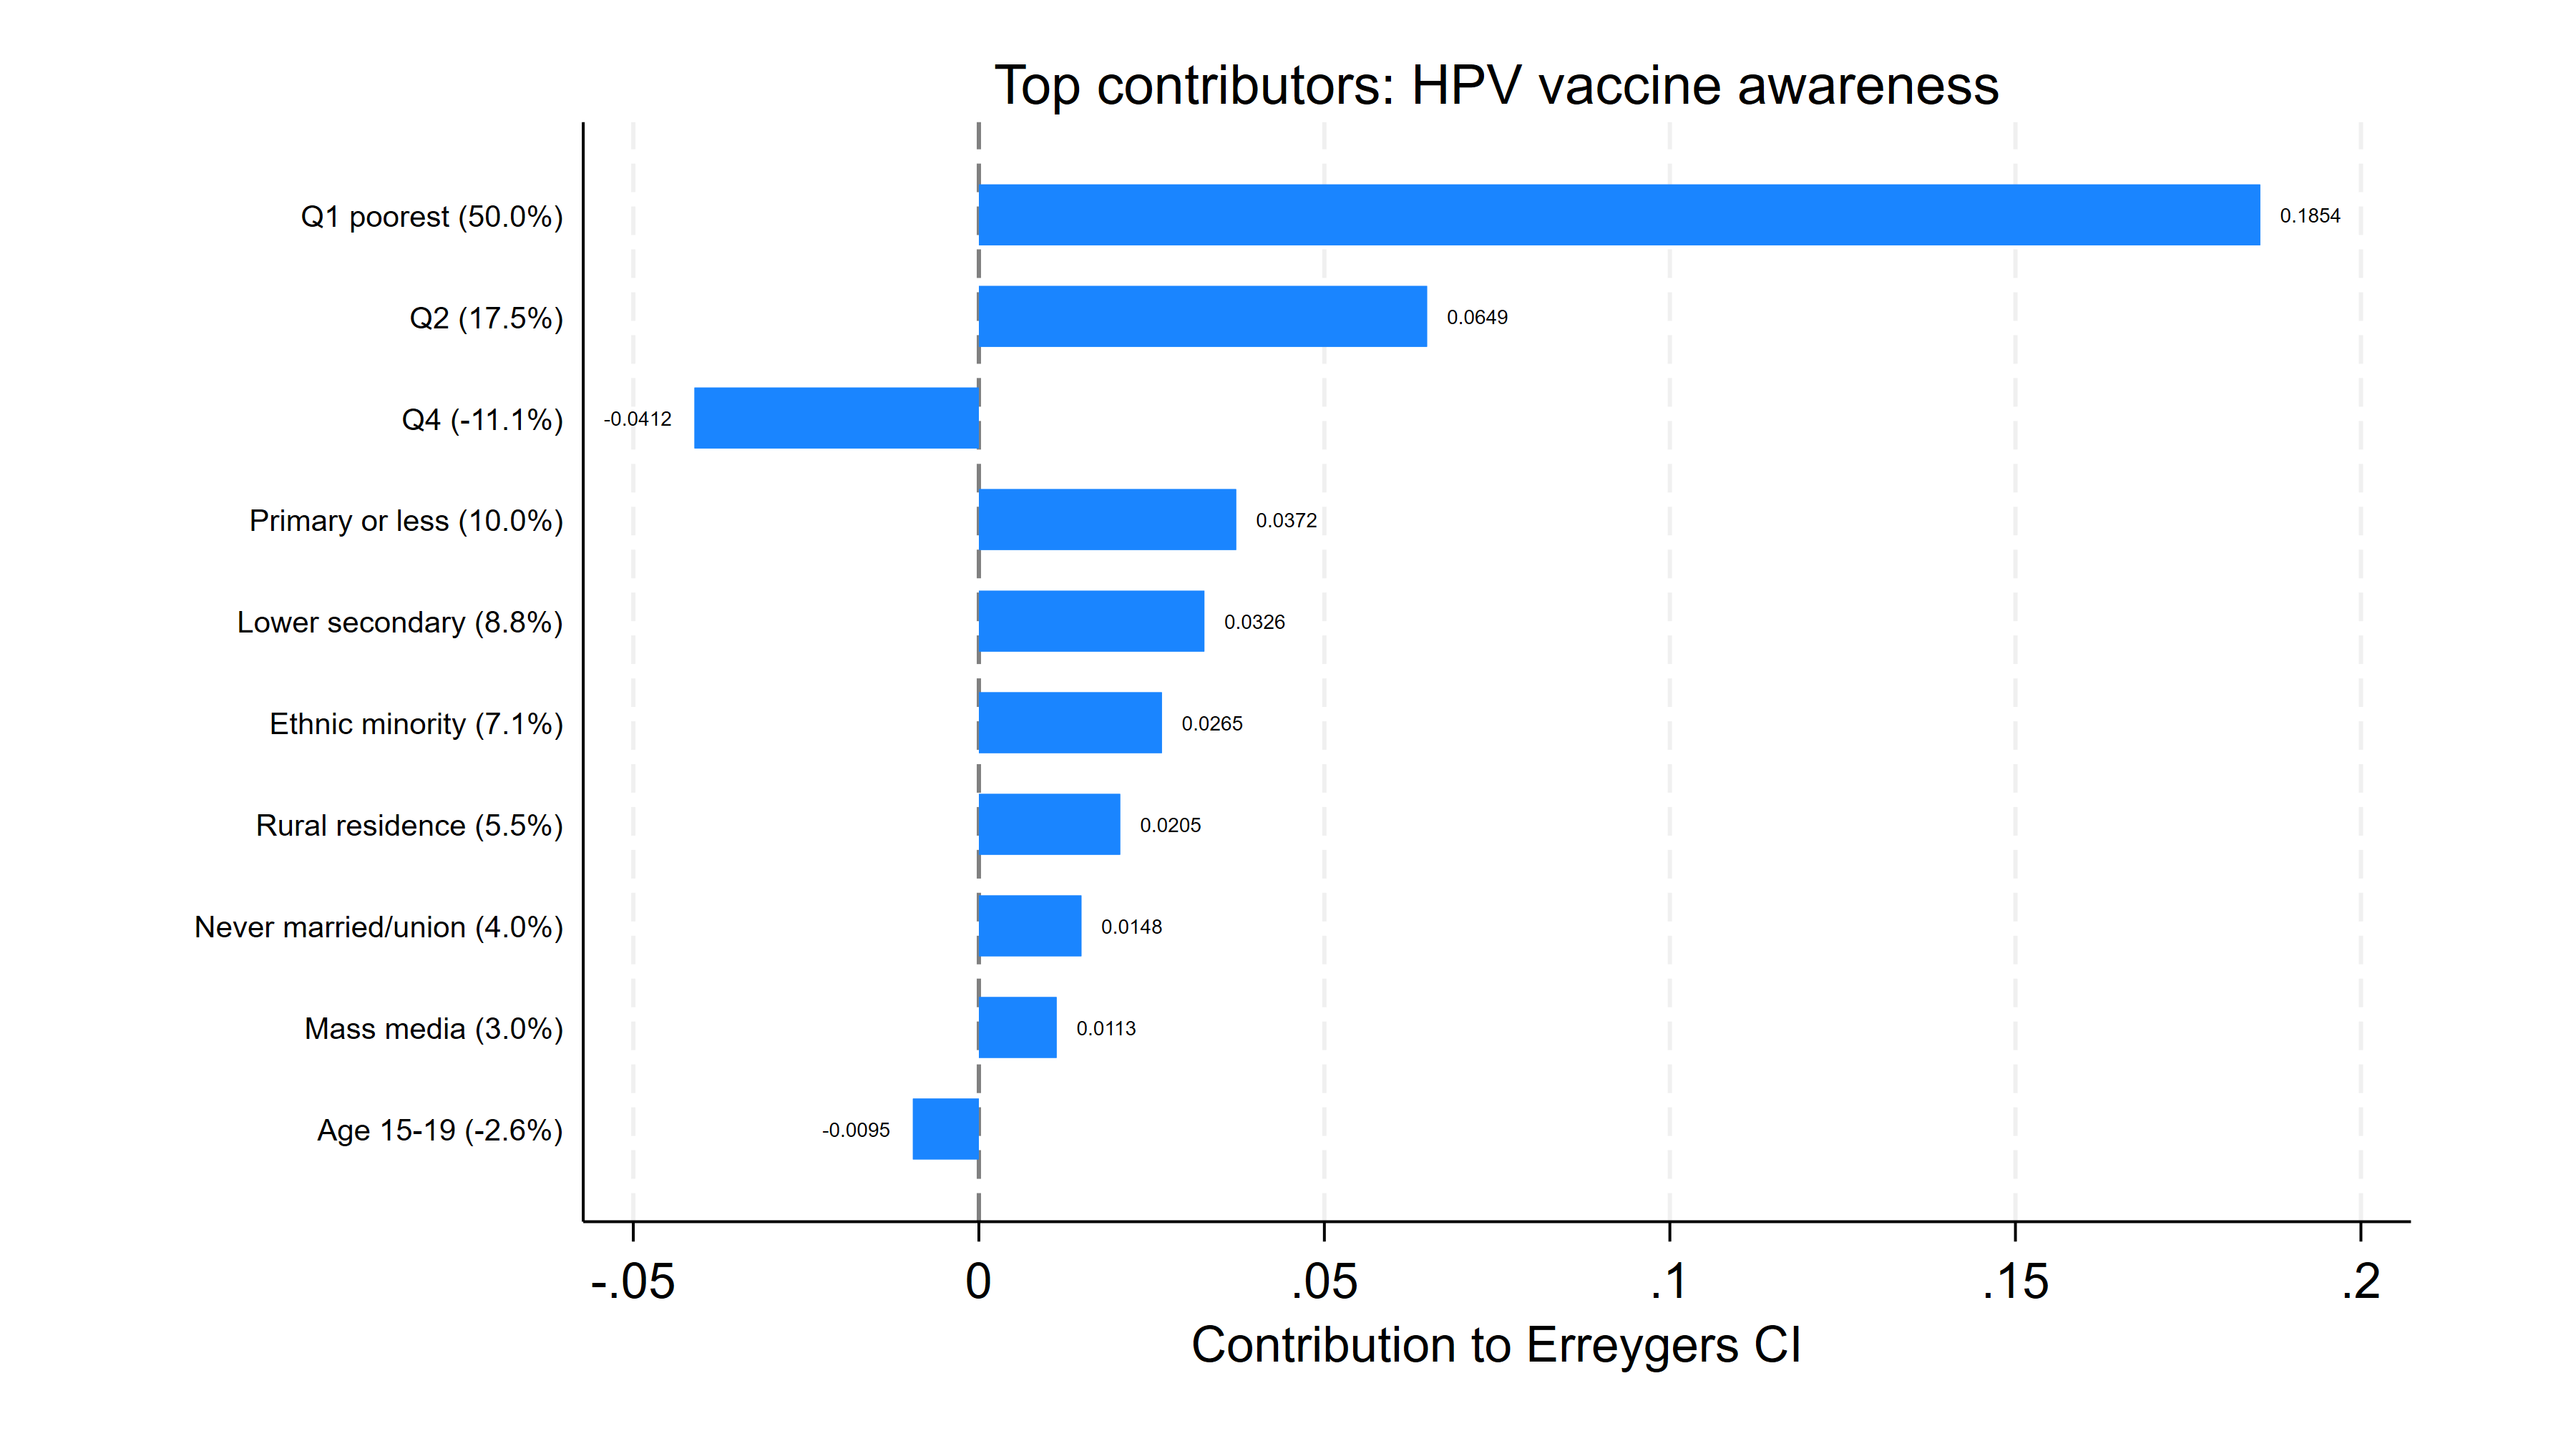
\includegraphics[width=0.90\textwidth]{Figures/fig8_decomposition_awareness.png}
\caption{Top contributors to socioeconomic inequality in HPV vaccine awareness.}
\label{fig:decomp_awareness}
\end{figure}

\begin{figure}[htbp]
\centering
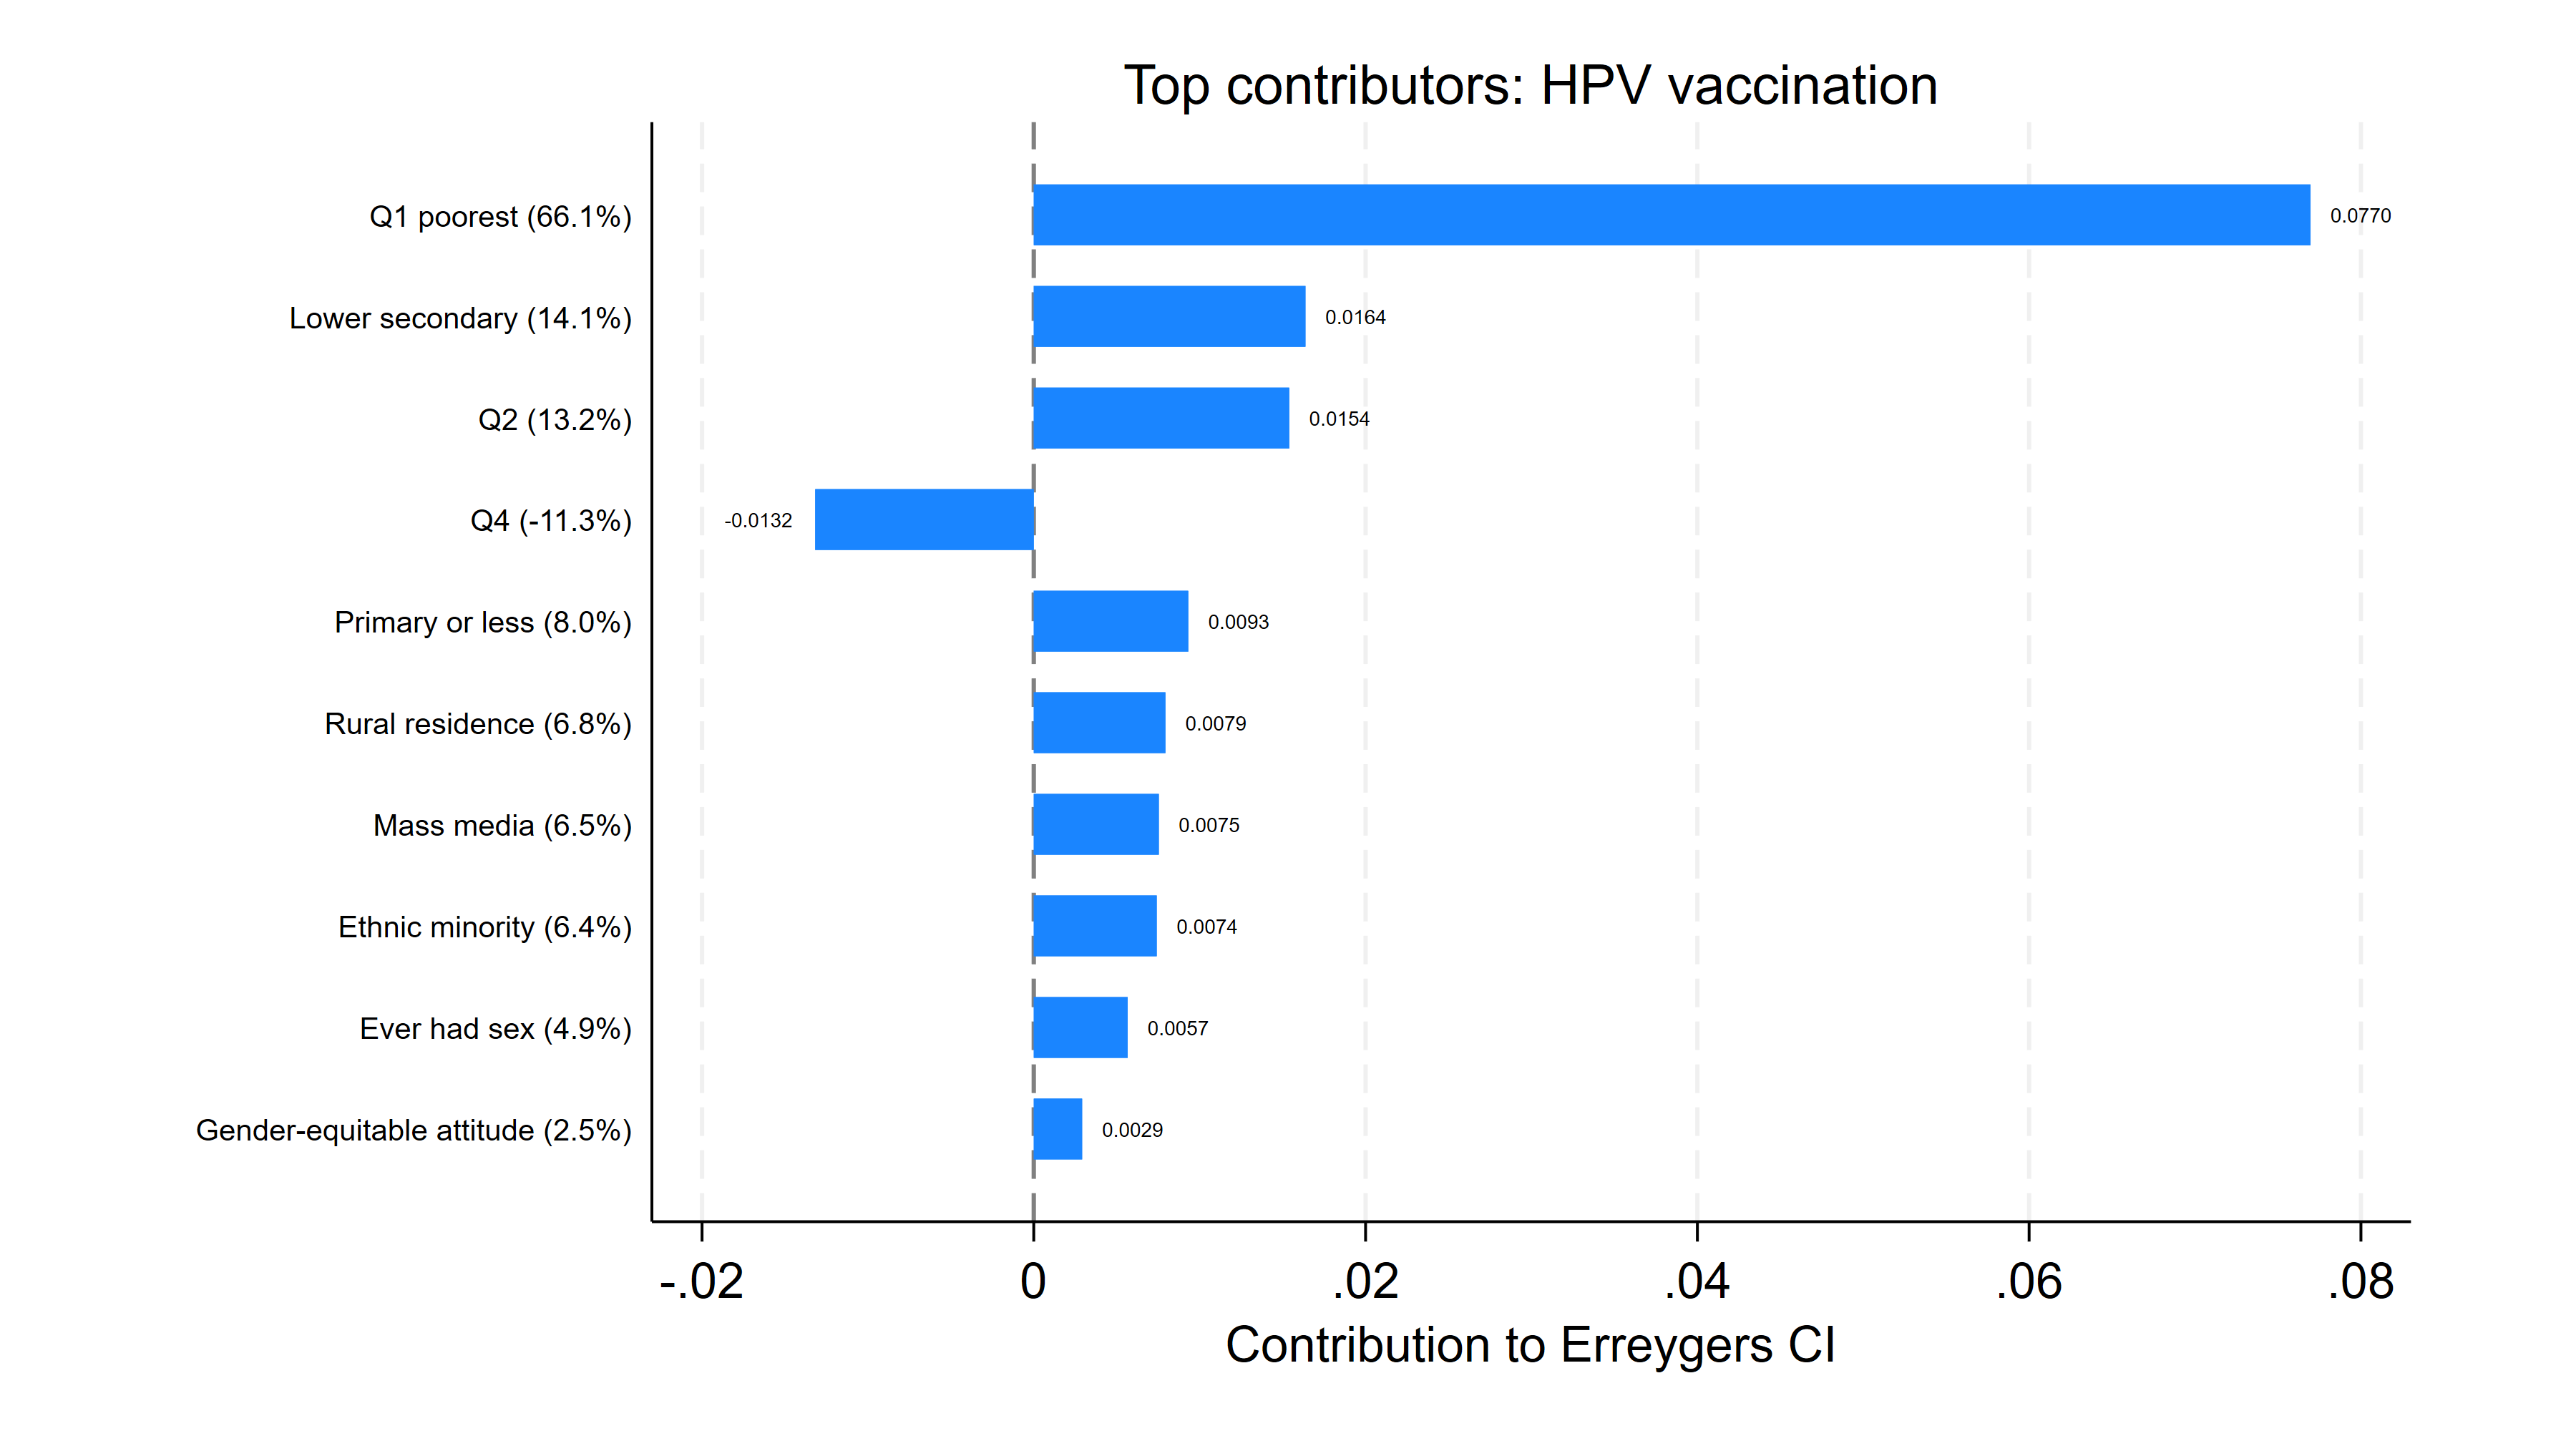
\includegraphics[width=0.90\textwidth]{Figures/fig9_decomposition_vaccination.png}
\caption{Top contributors to socioeconomic inequality in HPV vaccination.}
\label{fig:decomp_vaccination}
\end{figure}

\begin{figure}[htbp]
\centering
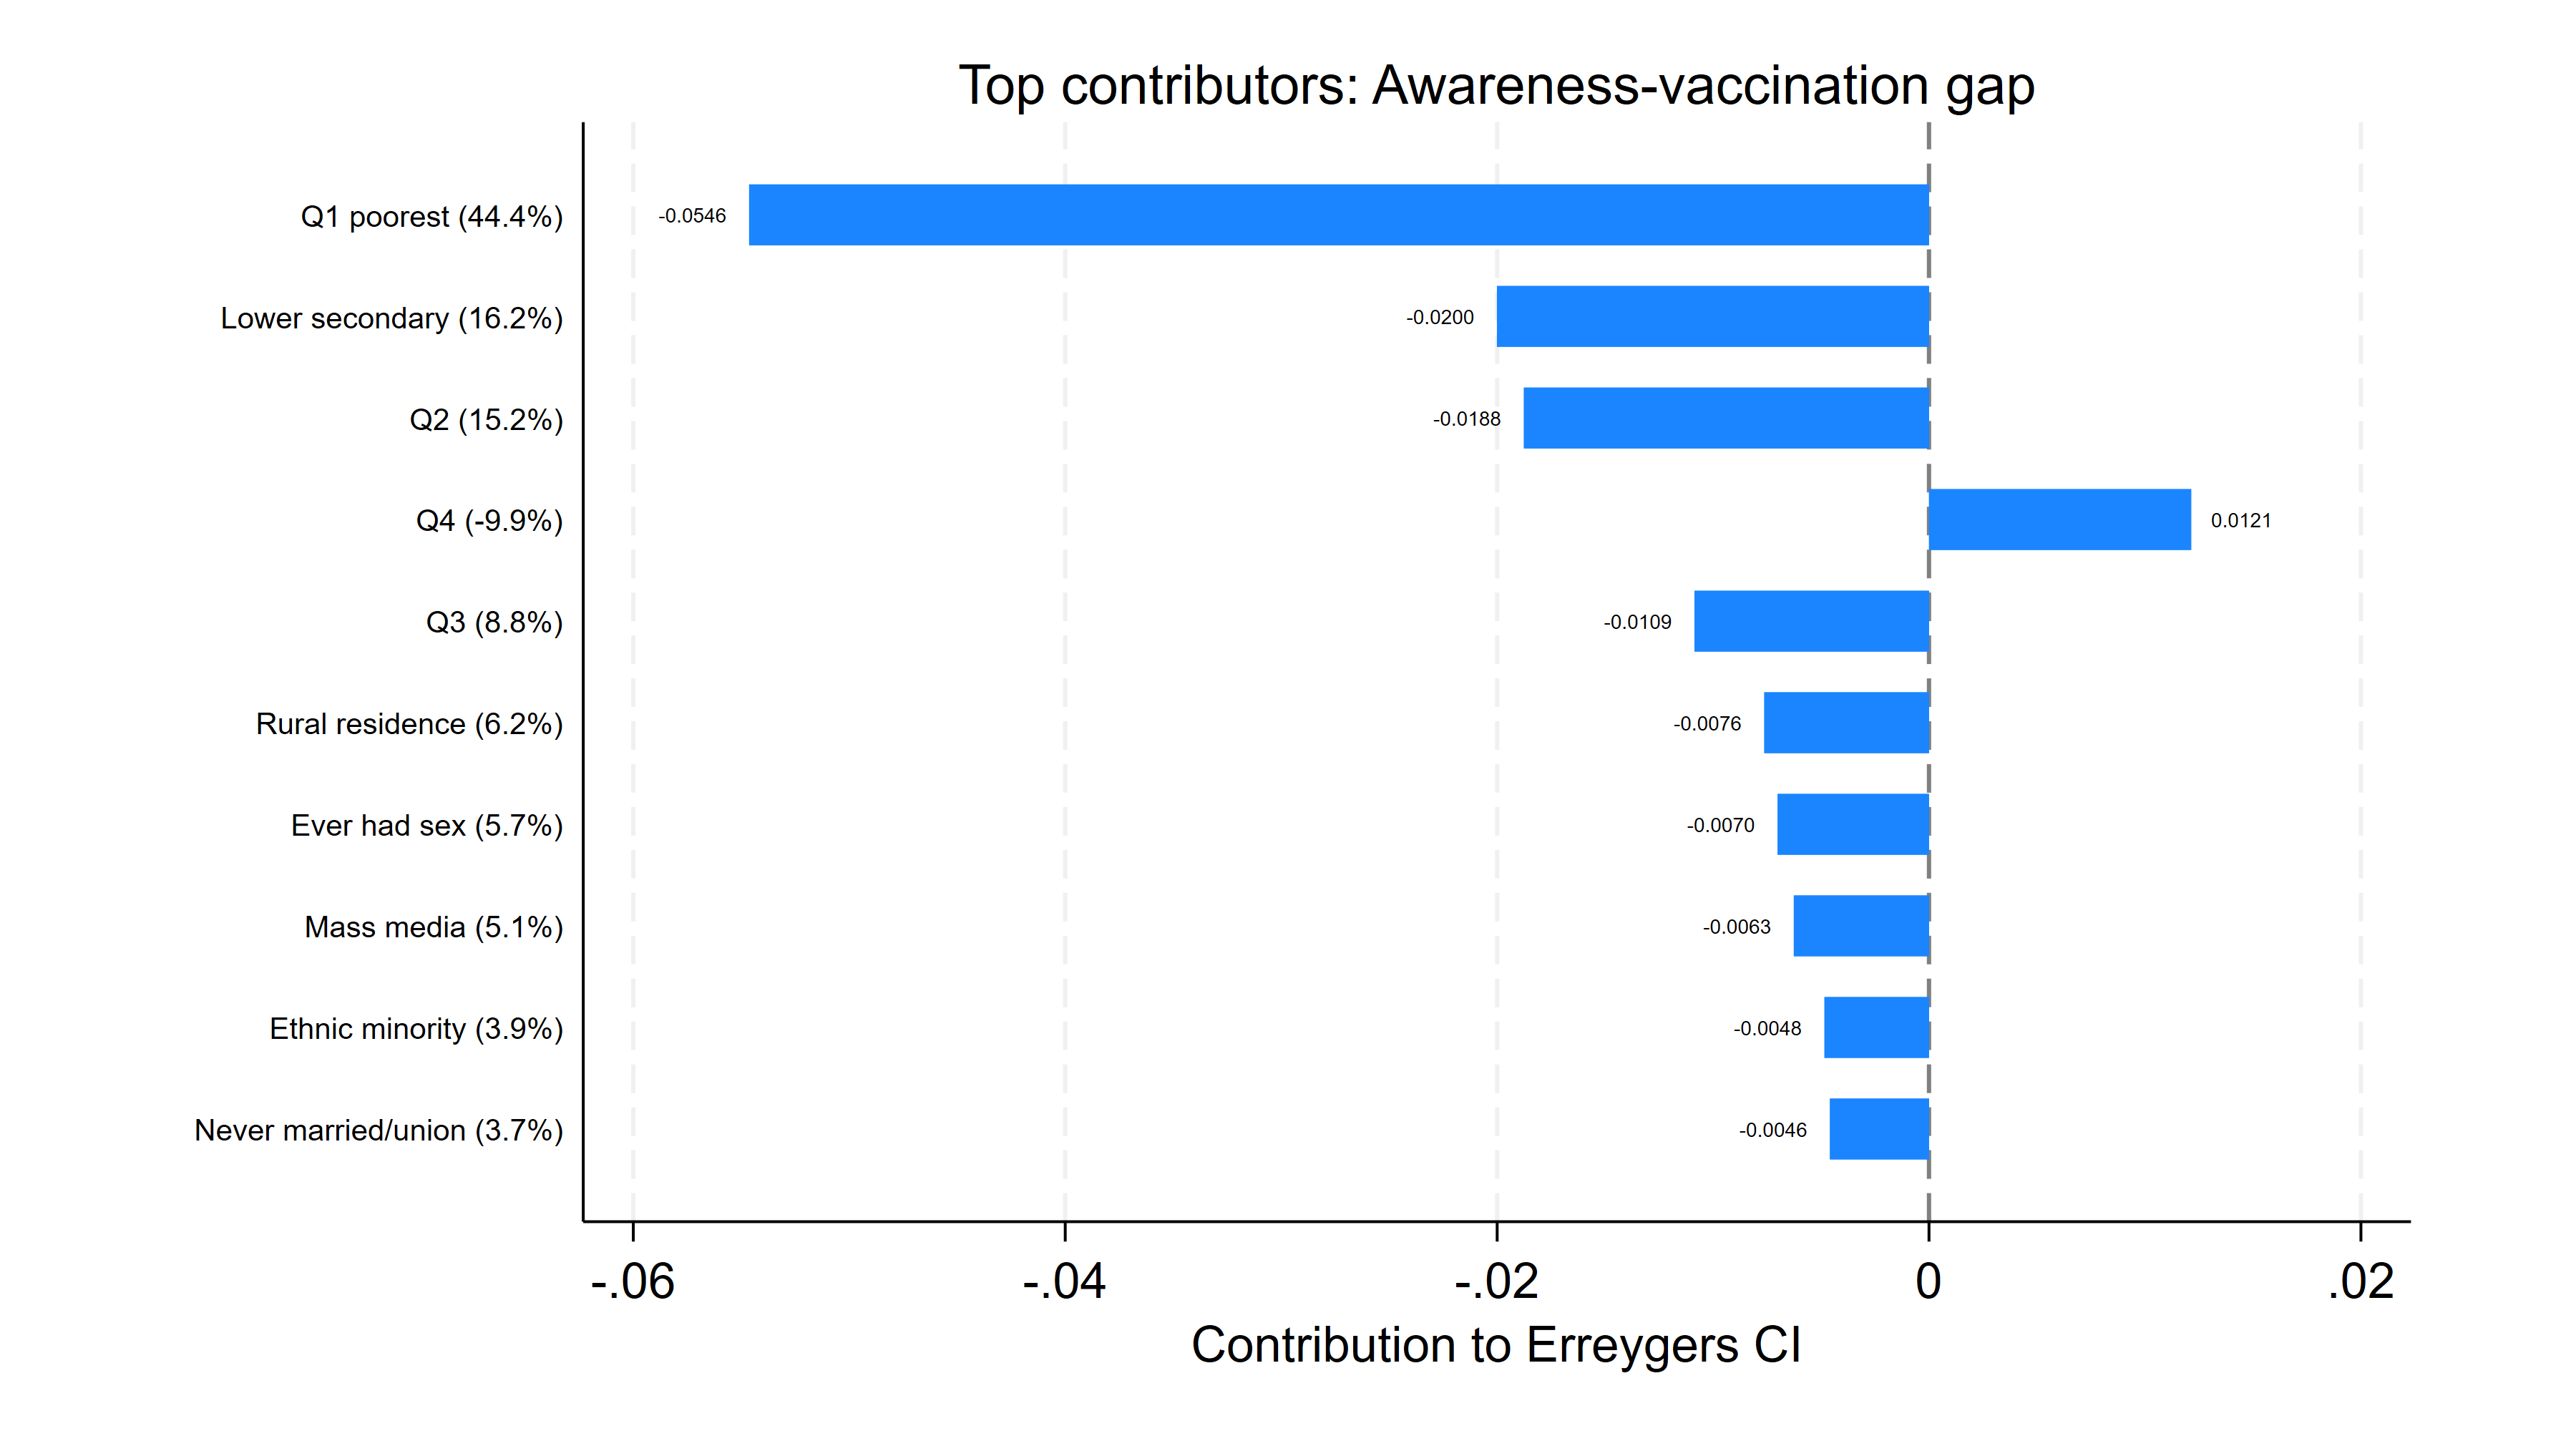
\includegraphics[width=0.90\textwidth]{Figures/fig10_decomposition_gap.png}
\caption[Awareness--vaccination gap decomposition]{Top contributors to socioeconomic inequality in the awareness--vaccination gap.}
\label{fig:decomp_gap}
\end{figure}

Because uncertainty intervals were not estimated for individual decomposition contributions, rankings should be interpreted as approximate descriptive accounting rather than statistically tested differences between contributors. In addition, wealth-quintile contributions are partly expected because the inequality rank is also based on household wealth; they describe how strongly the outcome gradient aligns with wealth groups rather than identifying wealth as an isolated causal mechanism. The decomposition indicates that wealth was central for both awareness and vaccination inequality. For awareness, the poorest wealth quintile, Q2, primary or lower secondary education, ethnic minority status, and rural residence were the largest contributors. For vaccination, the poorest quintile alone accounted for approximately two-thirds of the observed pro-rich inequality, followed by lower secondary education and Q2; Q4 had an offsetting negative contribution because it was less disadvantaged than the poorest groups but still below the richest reference group. For the gap, negative contributions from poorer wealth groups, lower secondary education, and rural residence were consistent with the pro-poor concentration of remaining unvaccinated among women who were already aware.

\clearpage
